%% bare_jrnl.tex
%% V1.4
%% 2012/12/27
%% by Michael Shell
%% see http://www.michaelshell.org/
%% for current contact information.
%%
%% This is a skeleton file demonstrating the use of IEEEtran.cls
%% (requires IEEEtran.cls version 1.8 or later) with an IEEE journal paper.
%%
%% Support sites:
%% http://www.michaelshell.org/tex/ieeetran/
%% http://www.ctan.org/tex-archive/macros/latex/contrib/IEEEtran/
%% and
%% http://www.ieee.org/



% *** Authors should verify (and, if needed, correct) their LaTeX system  ***
% *** with the testflow diagnostic prior to trusting their LaTeX platform ***
% *** with production work. IEEE's font choices can trigger bugs that do  ***
% *** not appear when using other class files.                            ***
% The testflow support page is at:
% http://www.michaelshell.org/tex/testflow/


%%*************************************************************************
%% Legal Notice:
%% This code is offered as-is without any warranty either expressed or
%% implied; without even the implied warranty of MERCHANTABILITY or
%% FITNESS FOR A PARTICULAR PURPOSE!
%% User assumes all risk.
%% In no event shall IEEE or any contributor to this code be liable for
%% any damages or losses, including, but not limited to, incidental,
%% consequential, or any other damages, resulting from the use or misuse
%% of any information contained here.
%%
%% All comments are the opinions of their respective authors and are not
%% necessarily endorsed by the IEEE.
%%
%% This work is distributed under the LaTeX Project Public License (LPPL)
%% ( http://www.latex-project.org/ ) version 1.3, and may be freely used,
%% distributed and modified. A copy of the LPPL, version 1.3, is included
%% in the base LaTeX documentation of all distributions of LaTeX released
%% 2003/12/01 or later.
%% Retain all contribution notices and credits.
%% ** Modified files should be clearly indicated as such, including  **
%% ** renaming them and changing author support contact information. **
%%
%% File list of work: IEEEtran.cls, IEEEtran_HOWTO.pdf, bare_adv.tex,
%%                    bare_conf.tex, bare_jrnl.tex, bare_jrnl_compsoc.tex,
%%                    bare_jrnl_transmag.tex
%%*************************************************************************

% Note that the a4paper option is mainly intended so that authors in
% countries using A4 can easily print to A4 and see how their papers will
% look in print - the typesetting of the document will not typically be
% affected with changes in paper size (but the bottom and side margins will).
% Use the testflow package mentioned above to verify correct handling of
% both paper sizes by the user's LaTeX system.
%
% Also note that the "draftcls" or "draftclsnofoot", not "draft", option
% should be used if it is desired that the figures are to be displayed in
% draft mode.
%
\documentclass[journal,UTF8]{IEEEtran}
\usepackage{color}
\usepackage{threeparttable}
%
% If IEEEtran.cls has not been installed into the LaTeX system files,
% manually specify the path to it like:
%\documentclass[journal]{../sty/IEEEtran}





% Some very useful LaTeX packages include:
% (uncomment the ones you want to load)


% *** MISC UTILITY PACKAGES ***
%
%\usepackage{ifpdf}
% Heiko Oberdiek's ifpdf.sty is very useful if you need conditional
% compilation based on whether the output is pdf or dvi.
% usage:
% \ifpdf
%   % pdf code
% \else
%   % dvi code
% \fi
% The latest version of ifpdf.sty can be obtained from:
% http://www.ctan.org/tex-archive/macros/latex/contrib/oberdiek/
% Also, note that IEEEtran.cls V1.7 and later provides a builtin
% \ifCLASSINFOpdf conditional that works the same way.
% When switching from latex to pdflatex and vice-versa, the compiler may
% have to be run twice to clear warning/error messages.






% *** CITATION PACKAGES ***
%
\usepackage{cite}
% cite.sty was written by Donald Arseneau
% V1.6 and later of IEEEtran pre-defines the format of the cite.sty package
% \cite{} output to follow that of IEEE. Loading the cite package will
% result in citation numbers being automatically sorted and properly
% "compressed/ranged". e.g., [1], [9], [2], [7], [5], [6] without using
% cite.sty will become [1], [2], [5]--[7], [9] using cite.sty. cite.sty's
% \cite will automatically add leading space, if needed. Use cite.sty's
% noadjust option (cite.sty V3.8 and later) if you want to turn this off
% such as if a citation ever needs to be enclosed in parenthesis.
% cite.sty is already installed on most LaTeX systems. Be sure and use
% version 4.0 (2003-05-27) and later if using hyperref.sty. cite.sty does
% not currently provide for hyperlinked citations.
% The latest version can be obtained at:
% http://www.ctan.org/tex-archive/macros/latex/contrib/cite/
% The documentation is contained in the cite.sty file itself.






% *** GRAPHICS RELATED PACKAGES ***
%
\ifCLASSINFOpdf
\usepackage[pdftex]{graphicx}
% declare the path(s) where your graphic files are
\graphicspath{{../pdf/}{../jpeg/}}
% and their extensions so you won't have to specify these with
% every instance of \includegraphics
\DeclareGraphicsExtensions{.pdf,.jpeg,.png}
\else
% or other class option (dvipsone, dvipdf, if not using dvips). graphicx
% will default to the driver specified in the system graphics.cfg if no
% driver is specified.
\usepackage[dvips]{graphicx}
% declare the path(s) where your graphic files are
\graphicspath{{../eps/}}
% and their extensions so you won't have to specify these with
% every instance of \includegraphics
\DeclareGraphicsExtensions{.eps}
\fi
% graphicx was written by David Carlisle and Sebastian Rahtz. It is
% required if you want graphics, photos, etc. graphicx.sty is already
% installed on most LaTeX systems. The latest version and documentation
% can be obtained at:
% http://www.ctan.org/tex-archive/macros/latex/required/graphics/
% Another good source of documentation is "Using Imported Graphics in
% LaTeX2e" by Keith Reckdahl which can be found at:
% http://www.ctan.org/tex-archive/info/epslatex/
%
% latex, and pdflatex in dvi mode, support graphics in encapsulated
% postscript (.eps) format. pdflatex in pdf mode supports graphics
% in .pdf, .jpeg, .png and .mps (metapost) formats. Users should ensure
% that all non-photo figures use a vector format (.eps, .pdf, .mps) and
% not a bitmapped formats (.jpeg, .png). IEEE frowns on bitmapped formats
% which can result in "jaggedy"/blurry rendering of lines and letters as
% well as large increases in file sizes.
%
% You can find documentation about the pdfTeX application at:
% http://www.tug.org/applications/pdftex





% *** MATH PACKAGES ***
%
\usepackage[cmex10]{amsmath}
% A popular package from the American Mathematical Society that provides
% many useful and powerful commands for dealing with mathematics. If using
% it, be sure to load this package with the cmex10 option to ensure that
% only type 1 fonts will utilized at all point sizes. Without this option,
% it is possible that some math symbols, particularly those within
% footnotes, will be rendered in bitmap form which will result in a
% document that can not be IEEE Xplore compliant!
%
% Also, note that the amsmath package sets \interdisplaylinepenalty to 10000
% thus preventing page breaks from occurring within multiline equations. Use:
%\interdisplaylinepenalty=2500
% after loading amsmath to restore such page breaks as IEEEtran.cls normally
% does. amsmath.sty is already installed on most LaTeX systems. The latest
% version and documentation can be obtained at:
% http://www.ctan.org/tex-archive/macros/latex/required/amslatex/math/





% *** SPECIALIZED LIST PACKAGES ***
%
%\usepackage{algorithmic}
\usepackage[ruled]{algorithm2e}
% algorithmic.sty was written by Peter Williams and Rogerio Brito.
% This package provides an algorithmic environment fo describing algorithms.
% You can use the algorithmic environment in-text or within a figure
% environment to provide for a floating algorithm. Do NOT use the algorithm
% floating environment provided by algorithm.sty (by the same authors) or
% algorithm2e.sty (by Christophe Fiorio) as IEEE does not use dedicated
% algorithm float types and packages that provide these will not provide
% correct IEEE style captions. The latest version and documentation of
% algorithmic.sty can be obtained at:
% http://www.ctan.org/tex-archive/macros/latex/contrib/algorithms/
% There is also a support site at:
% http://algorithms.berlios.de/index.html
% Also of interest may be the (relatively newer and more customizable)
% algorithmicx.sty package by Szasz Janos:
% http://www.ctan.org/tex-archive/macros/latex/contrib/algorithmicx/




% *** ALIGNMENT PACKAGES ***
%
\usepackage{array}

% Frank Mittelbach's and David Carlisle's array.sty patches and improves
% the standard LaTeX2e array and tabular environments to provide better
% appearance and additional user controls. As the default LaTeX2e table
% generation code is lacking to the point of almost being broken with
% respect to the quality of the end results, all users are strongly
% advised to use an enhanced (at the very least that provided by array.sty)
% set of table tools. array.sty is already installed on most systems. The
% latest version and documentation can be obtained at:
% http://www.ctan.org/tex-archive/macros/latex/required/tools/


% IEEEtran contains the IEEEeqnarray family of commands that can be used to
% generate multiline equations as well as matrices, tables, etc., of high
% quality.




% *** SUBFIGURE PACKAGES ***
\ifCLASSOPTIONcompsoc
\usepackage[caption=false,font=normalsize,labelfont=sf,textfont=sf]{subfig}
\else
\usepackage[caption=false,font=footnotesize]{subfig}
\fi
% subfig.sty, written by Steven Douglas Cochran, is the modern replacement
% for subfigure.sty, the latter of which is no longer maintained and is
% incompatible with some LaTeX packages including fixltx2e. However,
% subfig.sty requires and automatically loads Axel Sommerfeldt's caption.sty
% which will override IEEEtran.cls' handling of captions and this will result
% in non-IEEE style figure/table captions. To prevent this problem, be sure
% and invoke subfig.sty's "caption=false" package option (available since
% subfig.sty version 1.3, 2005/06/28) as this is will preserve IEEEtran.cls
% handling of captions.
% Note that the Computer Society format requires a larger sans serif font
% than the serif footnote size font used in traditional IEEE formatting
% and thus the need to invoke different subfig.sty package options depending
% on whether compsoc mode has been enabled.
%
% The latest version and documentation of subfig.sty can be obtained at:
% http://www.ctan.org/tex-archive/macros/latex/contrib/subfig/




% *** FLOAT PACKAGES ***
%
%\usepackage{fixltx2e}
% fixltx2e, the successor to the earlier fix2col.sty, was written by
% Frank Mittelbach and David Carlisle. This package corrects a few problems
% in the LaTeX2e kernel, the most notable of which is that in current
% LaTeX2e releases, the ordering of single and double column floats is not
% guaranteed to be preserved. Thus, an unpatched LaTeX2e can allow a
% single column figure to be placed prior to an earlier double column
% figure. The latest version and documentation can be found at:
% http://www.ctan.org/tex-archive/macros/latex/base/


%\usepackage{stfloats}
% stfloats.sty was written by Sigitas Tolusis. This package gives LaTeX2e
% the ability to do double column floats at the bottom of the page as well
% as the top. (e.g., "\begin{figure*}[!b]" is not normally possible in
% LaTeX2e). It also provides a command:
%\fnbelowfloat
% to enable the placement of footnotes below bottom floats (the standard
% LaTeX2e kernel puts them above bottom floats). This is an invasive package
% which rewrites many portions of the LaTeX2e float routines. It may not work
% with other packages that modify the LaTeX2e float routines. The latest
% version and documentation can be obtained at:
% http://www.ctan.org/tex-archive/macros/latex/contrib/sttools/
% Do not use the stfloats baselinefloat ability as IEEE does not allow
% \baselineskip to stretch. Authors submitting work to the IEEE should note
% that IEEE rarely uses double column equations and that authors should try
% to avoid such use. Do not be tempted to use the cuted.sty or midfloat.sty
% packages (also by Sigitas Tolusis) as IEEE does not format its papers in
% such ways.
% Do not attempt to use stfloats with fixltx2e as they are incompatible.
% Instead, use Morten Hogholm'a dblfloatfix which combines the features
% of both fixltx2e and stfloats:
%
% \usepackage{dblfloatfix}
% The latest version can be found at:
% http://www.ctan.org/tex-archive/macros/latex/contrib/dblfloatfix/




%\ifCLASSOPTIONcaptionsoff
%  \usepackage[nomarkers]{endfloat}
% \let\MYoriglatexcaption\caption
% \renewcommand{\caption}[2][\relax]{\MYoriglatexcaption[#2]{#2}}
%\fi
% endfloat.sty was written by James Darrell McCauley, Jeff Goldberg and
% Axel Sommerfeldt. This package may be useful when used in conjunction with
% IEEEtran.cls'  captionsoff option. Some IEEE journals/societies require that
% submissions have lists of figures/tables at the end of the paper and that
% figures/tables without any captions are placed on a page by themselves at
% the end of the document. If needed, the draftcls IEEEtran class option or
% \CLASSINPUTbaselinestretch interface can be used to increase the line
% spacing as well. Be sure and use the nomarkers option of endfloat to
% prevent endfloat from "marking" where the figures would have been placed
% in the text. The two hack lines of code above are a slight modification of
% that suggested by in the endfloat docs (section 8.4.1) to ensure that
% the full captions always appear in the list of figures/tables - even if
% the user used the short optional argument of \caption[]{}.
% IEEE papers do not typically make use of \caption[]'s optional argument,
% so this should not be an issue. A similar trick can be used to disable
% captions of packages such as subfig.sty that lack options to turn off
% the subcaptions:
% For subfig.sty:
% \let\MYorigsubfloat\subfloat
% \renewcommand{\subfloat}[2][\relax]{\MYorigsubfloat[]{#2}}
% However, the above trick will not work if both optional arguments of
% the \subfloat command are used. Furthermore, there needs to be a
% description of each subfigure *somewhere* and endfloat does not add
% subfigure captions to its list of figures. Thus, the best approach is to
% avoid the use of subfigure captions (many IEEE journals avoid them anyway)
% and instead reference/explain all the subfigures within the main caption.
% The latest version of endfloat.sty and its documentation can obtained at:
% http://www.ctan.org/tex-archive/macros/latex/contrib/endfloat/
%
% The IEEEtran \ifCLASSOPTIONcaptionsoff conditional can also be used
% later in the document, say, to conditionally put the References on a
% page by themselves.




% *** PDF, URL AND HYPERLINK PACKAGES ***
%
%\usepackage{url}
% url.sty was written by Donald Arseneau. It provides better support for
% handling and breaking URLs. url.sty is already installed on most LaTeX
% systems. The latest version and documentation can be obtained at:
% http://www.ctan.org/tex-archive/macros/latex/contrib/url/
% Basically, \url{my_url_here}.




% *** Do not adjust lengths that control margins, column widths, etc. ***
% *** Do not use packages that alter fonts (such as pslatex).         ***
% There should be no need to do such things with IEEEtran.cls V1.6 and later.
% (Unless specifically asked to do so by the journal or conference you plan
% to submit to, of course. )


% correct bad hyphenation here
\hyphenation{op-tical net-works semi-conduc-tor}



\begin{document}
	%
	% paper title
	% can use linebreaks \\ within to get better formatting as desired
	% Do not put math or special symbols in the title.
	\title{A User-oriented Development Method \textcolor{red}{in Multiprocessor Embedded PLCs for Complex Logic and Motion Control Mixed Scenarios}}
	% * <larryb@accdon.com> 2018-08-30T22:43:46.755Z:
	% 
	% > FSM supported Multiprocessor Embedded PLCs
	% Author - Please spell out acronyms in titles.
	% 
	% ^.
	%
	%
	% author names and IEEE memberships
	% note positions of commas and nonbreaking spaces ( ~ ) LaTeX will not break
	% a structure at a ~ so this keeps an author's name from being broken across
	% two lines.
	% use \thanks{} to gain access to the first footnote area
	% a separate \thanks must be used for each paragraph as LaTeX2e's \thanks
	% was not built to handle multiple paragraphs
	%
	
	
	
	% note the % following the last \IEEEmembership and also \thanks -
	% these prevent an unwanted space from occurring between the last author name
	% and the end of the author line. i.e., if you had this:
	%
	% \author{....lastname \thanks{...} \thanks{...} }
	%                     ^------------^------------^----Do not want these spaces!
	%
	% a space would be appended to the last name and could cause every name on that
	% line to be shifted left slightly. This is one of those "LaTeX things". For
	% instance, "\textbf{A} \textbf{B}" will typeset as "A B" not "AB". To get
	% "AB" then you have to do: "\textbf{A}\textbf{B}"
	% \thanks is no different in this regard, so shield the last } of each \thanks
	% that ends a line with a % and do not let a space in before the next \thanks.
	% Spaces after \IEEEmembership other than the last one are OK (and needed) as
	% you are supposed to have spaces between the names. For what it is worth,
	% this is a minor point as most people would not even notice if the said evil
	% space somehow managed to creep in.
	
	
	
	% The paper headers
	
	%\markboth{Journal of \LaTeX\ Class Files,~Vol.~11, No.~4, December~2012}%
	%{Shell \MakeLowercase{\textit{et al.}}: Bare Demo of IEEEtran.cls for Journals}
	
	% The only time the second header will appear is for the odd numbered pages
	% after the title page when using the twoside option.
	%
	% *** Note that you probably will NOT want to include the author's ***
	% *** name in the headers of peer review papers.                   ***
	% You can use \ifCLASSOPTIONpeerreview for conditional compilation here if
	% you desire.
	
	
	
	
	% If you want to put a publisher's ID mark on the page you can do it like
	% this:
	%\IEEEpubid{0000--0000/00\$00.00~\copyright~2012 IEEE}
	% Remember, if you use this you must call \IEEEpubidadjcol in the second
	% column for its text to clear the IEEEpubid mark.
	
	
	
	% use for special paper notices
	%\IEEEspecialpapernotice{(Invited Paper)}
	
	
	
	
	% make the title area
	\maketitle
	
	
	\begin{abstract}
		\textcolor{red}{Programmable logic controllers ($PLC$s) are a foundation of automation, but applications become complex in logic and motion control mixed scenarios, while a PC-based $PLC$ incurs a high monetary cost and comprises a complex system that cannot meet the customized requirements of large equipment. The development of $PLC$s has encountered bottlenecks. Hence, in this paper, we theoretically present a user-oriented development method containing a comprehensive optimization method. In practice, we implement this concept by proposing a customized multiprocessor embedded $PLC$ ($ePLC$) to enhance the performance, a multi-language supported uniform development platform to improve the adaptability of developers, and an optimized system structure (reasonable memory allocation, user-oriented thread structure, proposed $LPM$ data interaction, modular software design, and finite state machines) to reduce the development complexity.} Ultimately, we adopt the proposed method to implement a distributed control system on a 200-T injection molding machine. Through comparison with TECHMATION and KEBA systems, the startup time of the implemented system was increased by more than 5 times, while the key performance is almost identical. In addition, the implemented system adopts the customized multiprocessor embeded $PLC$ and detached human machine interface ($HMI$).
		% * <larryb@accdon.com> 2018-08-30T22:48:45.543Z:
		% 
		% > $ePLC$
		% Author - Please explain the designation ePLC.
		% 
		% ^.
		
	\end{abstract}
	
	% Note that keywords are not normally used for peerreview papers.
	\begin{IEEEkeywords}
		Multiprocessor, motion control, injection molding machine, embedded PLC, user-oriented
	\end{IEEEkeywords}
	
	% For peer review papers, you can put extra information on the cover
	% page as needed:
	% \ifCLASSOPTIONpeerreview
	% \begin{center} \bfseries EDICS Category: 3-BBND \end{center}
	% \fi
	%
	% For peerreview papers, this IEEEtran command inserts a page break and
	% creates the second title. It will be ignored for other modes.
	\IEEEpeerreviewmaketitle
	
	
	
	\section{Introduction}
	Some concepts, such as smart factory and intelligent manufacturing \cite{Chekired2018Industrial,cheng2018industrial}, and some technologies, such as the Internet of Things, 5G, and augmented reality \textcolor{red}{\cite{da2014internet,Liu2016Traversing,Li20185G}}, are paving the road of the fourth industrial revolution. Normally, a typical plant is full of large equipment; for instance, cranes, computerized numerical control (CNC) machining centers, injection molding machines ($IMM$s), air pumps, chillers, automatic-guided vehicles, and various types of robots, and most of them are controlled by programmable logic controllers ($PLC$s), which have become a primary control system. Numerous researchers are focusing on $PLC$ technologies that significantly extend the application fields of PLCs. \cite{Jiang2013System,Jiang2013Bayesian,Adiego2015Applying} guaranteed PLC reliability by verifying their programming, \cite{Gerk2006Advanced,Chang2007Adaptive,Dominic2016PLC} improved the performance of $PLC$s using advanced algorithms, \cite{wu2018customized} alleviated the development complexity of $PLC$s using special software structure, and \cite{Sch2013Development,Morenas2017Shop} proposed methods of updating $PLCs$ programs dynamically.
	% * <larryb@accdon.com> 2018-08-30T22:53:37.974Z:
	% 
	% > CNC
	% Author - Please define this acronym.
	% 
	% ^.
	However, with the rapidly growing demand for, and the trends of, applications to be user-oriented and mix complex logic and motion control\cite{Zaeh2005A,Hossain2014Advanced}, $PLC$s still encounter bottlenecks, especially on large equipment (CNC machining centers, $IMMs$, etc.).
	
	\subsection{Motivations}
	Currently, the hardware architecture of $PLC$s can take two directions: embedded $PLC$s ($ePLC$s) and PC-based $PLC$s. PC-based $PLC$s are increasingly used in applications of complex logic and motion control mixed scenarios on account of its high performance and numerous user-oriented tools \cite{Hossain2014Advanced}. Considering the IMM industry, Table \ref{table:IMMSystem} lists the composition of IMMs, including parts (described as modules for programming), digital input$\backslash$output (DI$\backslash$Os), and analog input$\backslash$output (AI$\backslash$Os). Normally, the simplest IMM system consists of 10 modules, 20 DIs, 30 DOs, three AIS, and seven AOs. Complex relations among them and the high-performance requirements of algorithms tremendously increase the difficulty of programming. Hence, as listed in Table \ref{table:IMMControllor}, a comparison of KEBA, BECKHOFF, GAFRAN, and TECKMATION systems, which are the main brands of IMM controllers, illustrates that almost all of them use PC-based PLCs. \textcolor{red}{In the PC-based $PLC$, the runtime executes in some cumbersome systems (e.g., VxWorks, Windows CE, RTLinux). Additionally considering the above-mentioned complexity of an $IMM$ system and the software architecture of PC-based $PLC$s, it has become a huge project to build their own $IMM$ system for the manufacturers; hence, the hardware and software of the controller are always fixed and the $HMI$ is also integrated with the $PLC$. This situation leads to little independence among $IMM$ manufacturers and the development of $PLC$s in these scenarios has encountered bottlenecks.}

	

	$ePLC$s have a wide area of application in automation due to their easy programming and high reliability, \textcolor{red}{which induces a large paradigm shift of $PLCs$ to the embedded processor market. Some Platforms (e.g., OpenPLC \cite{alves2014openplc}) are transferred to some market-friendly embedded hardware (e.g., Raspberry-Pi) to improve acceptability. Some light-weight operating systems (e.g., uClinux \cite{gaur2015operating}) are adopted in embedded processors to simplify the development of an embedded system. Some methods, such as model- and component-based software \cite{Bonf2013Design, Vyatkin2013Software}, have also been researched to reduce the complexity of $PLC$ programs.
%	Advances in fields such as wireless communication and the Internet of Things \cite{Arshad2017Green} have an accelerated requirement for $ePLC$s. 
	However, some disadvantages still limit its further development \cite{Hossain2014Advanced}, especially when coping with complex logic and motion control mixed applications. A more comprehensively improved development method combining these above-mentioned advances still should be proposed. Hence, how to integrate easy programming and the high reliability of $ePLCs$ with high performance becomes crucial for logic and motion control mixed scenarios.}
	
	\subsection{Related Works}
	\textcolor{red}{To address the problem of complex logic and motion control mixed scenarios,} various researchers have presented methods of integrating motion control algorithms (e.g., linear interpolation, position control, arc interpolation, etc.) into $PLC$s \cite{Shi2016The,Fang2017Design},  and thus logic control and motion control become inseparable. There are two ways to realize this integration: 1) an individual motion control module integrated with the $PLC$ \cite{Peng2011Linear}, and 2) $PLC$s featuring motion control functions \textcolor{red}{\cite{syaichu2011model,kapernick2014plc,ruting2016model}}. Regarding an individual motion control module, different kinds of modules and $PLC$s coded in different languages and developed on their own platforms tremendously increase the complexity of implementing applications. \cite{Peng2011Linear,Qian2014A,Panasonic2011Programmable} all describe these modules. The second way simplifies the development method; nevertheless, it is difficult to guarantee high-reliability logic control and high-accuracy motion control simultaneously, since they run in the same thread. 
	
	We propose the concept of a multiprocessor $ePLC$ (multiple processor chips and multiple cores in one chip are all called multiprocessors in this paper). In this $ePLC$, extra processors (e.g., DSP, FPGA, etc.) are introduced to enhance performance. Various technologies contribute to the improvement of multiple processors. \cite{Dubois2002Memory,Patel2006Processor} proposed data-interaction methods among multiple processors, \cite{Zhu2016Providing} presented a method to balance the computing ability of the processors, \cite{Albarakat2017MTB} proposed a thread-scheduling method in multiprocessors. All of these works are not implemented in the $ePLC$, but have inspired us to build the architecture of a multiprocessor $ePLC$. Moreover, some research \cite{Hajduk2015Architecture, Chmiel2016An} introduced additional high-performance processors into $ePLC$s, although no improvement in the development method was proposed for complex logic and motion control mixed applications.
	
	In terms of the development methods of the individual module, which is very convoluted, users should take considerable time in selecting the platform and additional time in learning the particular software and its supported language. For instance, PMAC uses C++ \cite{Peng2011Linear,Qian2014A}, MC421/221 of the OMRON CS1 series is supported by G-Code \cite{OMRON2006CS1W}, the FP series $PLC$ of Panasonic adopts special instructions embedded in  a ladder diagram (LD). Therefore, the uniform development methodology in $PLC$ platforms has attracted our interest. Since the 1990s, IEC-61131 has been focused on the standardization of $PLC$s \cite{IEC1993Programmable}. In 2005, the PLCopen organization released a related standard \cite{PLCopen2005Function} that standardizes the motion control in $PLC$s and then publications, such as \cite{S2006Advanced}, suggested interactions using it, and companies, such as 3S \cite{3S2017Logic}, provided some tools. However, regarding such complex applications, programmers occasionally prefer to use more popular or object-oriented languages (e.g., C, C++, etc.) \cite{Bonfe2001Object, Werner2009Object, Basile2013On}, rather than the languages specified in IEC-61131-3. 
	
	
	\subsection{Our Contributions}
	\textcolor{red}{Considering the popular user-oriented concept \cite{Verscheure2016User, Choi2017A}, in this work we theoretically develop a concept of a user-oriented development method. To the best of our knowledge, a user-oriented development method should improve every aspect of the $PLC$ system (development method, program, processor, $RAM$, and threading) and contain a comprehensive optimization approach \textbf{to address specific problems from the user's point of view}.} Hence, we pose a flexible solution to enhance performance by adding sufficient processors, a multi-language-supported graphical component to improve the adaptability of developers, an optimized system structure (reasonable memory allocation, user-oriented thread structure, $LPM$ data interaction, modular software design, and finite state machines) to reduce the development complexity. Ultimately, we adopt the proposed method to implement a distributed $IMM$ system that is considered a kind of complex logic and motion control mixed application.
	
	This rest of this paper is organized as follows. In Section \ref{MultiProcessorePLC}, we introduce the system architecture, multi-language supported graphical component, memory allocation, user-oriented multi-threading, and modular design. In Section \ref{Process}, we present the compilation of graphical components, the $LPM$ data interaction mechanism, the execution of multi-threading, and finite state machines. Finally, in section \ref{Experiment}, we implement the $IMM$ distributed system with the proposed method and compare it with the TECHMATION and KEBA systems from aspects of system condition, system structure, and key performance.
	\begin{table}
		\scriptsize \caption{Modules, DI/DO, AI/AO of $IMM$}
		\label{table:IMMSystem}
		\begin{center}
			\renewcommand{\arraystretch}{1.4}
			\setlength\tabcolsep{3pt}
			\begin{tabular}{|p{0.3cm}|p{0.8cm}|p{1.8cm}|p{1.2cm}|p{1.8cm}|p{1.7cm}|}
				\hline
				No. & Module      & DI                       & DO           & AI                     & AO\\
				\hline
				1  & Mold       & Safety valve & Mold close     & Mold position        &System pressure \\
				\hline
				2  & Injection  & Heating detection & Mold open      & Injection position    &System flow\\
				\hline
				3  & Core      & Servo alarm         & Inject          & Nozzle position      &Back pressure\\
				\hline
				4  & Nozzle    & Motor overload            & Charging         & Temperature 1        &  \\
				\hline
				5  & Heating   & Emergency button           & Grean light       & Temperature 2        &\\
				\hline
				6  & Ejector   & Injection shield          & Red light         & Temperature 3       &\\
				\hline
				7  & AirValve & Detection switch          & Yellow light       & Temperature 4      &\\
				\hline
				...  & ....        & ...                       & ...                & ...                &...\\
				\hline
				50  &             & Screw speed                &                    &                     & \\
				\hline
			\end{tabular}
		\end{center}
	\end{table}
	\begin{table}
		\scriptsize \caption{System Comparison of PC-Based $PLC$ in $IMM$}
		\label{table:IMMControllor}
		\begin{center}
			\renewcommand{\arraystretch}{1.4}
			\setlength\tabcolsep{3pt}
			\begin{tabular}{|p{1.6cm}|p{1cm}|p{1.2cm}|p{1.4cm}|p{1.1cm}|p{1.3cm}|}
				\hline
				Brand       & CPU       & System & Language       & Distributed & HMI\\
				\hline
				TECHMATION  & DSP       & -  & Assembly  &No           & Irreplaceable \\
				\hline
				KEBA        & PC-based  &VxWorks   & IEC61131-3   &Yes          & Irreplaceable\\
				\hline
				BECKHOFF    & PC-Based  &WindowsCE & IEC61131-3  &Yes          &Irreplaceable\\
				\hline
				GEFRAN      & PC-based  &VxWorks   &IEC61131-3     &Yes          &Irreplaceable\\
				\hline
			\end{tabular}
		\end{center}
	\end{table}
	\section{System Architecture}
	\label{MultiProcessorePLC}
	\subsection{Hardware Structure of $ePLC$}
	Figure \ref{fig:HardwareStructure} shows one type of hardware structure of a multiprocessor $ePLC$ that contains a master processor and two slave processors. The master processor is responsible for logic control, communication, etc. The slave processor is designed for complex algorithms that can be customized on demand (the number of processors, DI$\backslash$Os, AI$\backslash$Os, and controlled servo motors).
	\begin{figure}
		\centering
		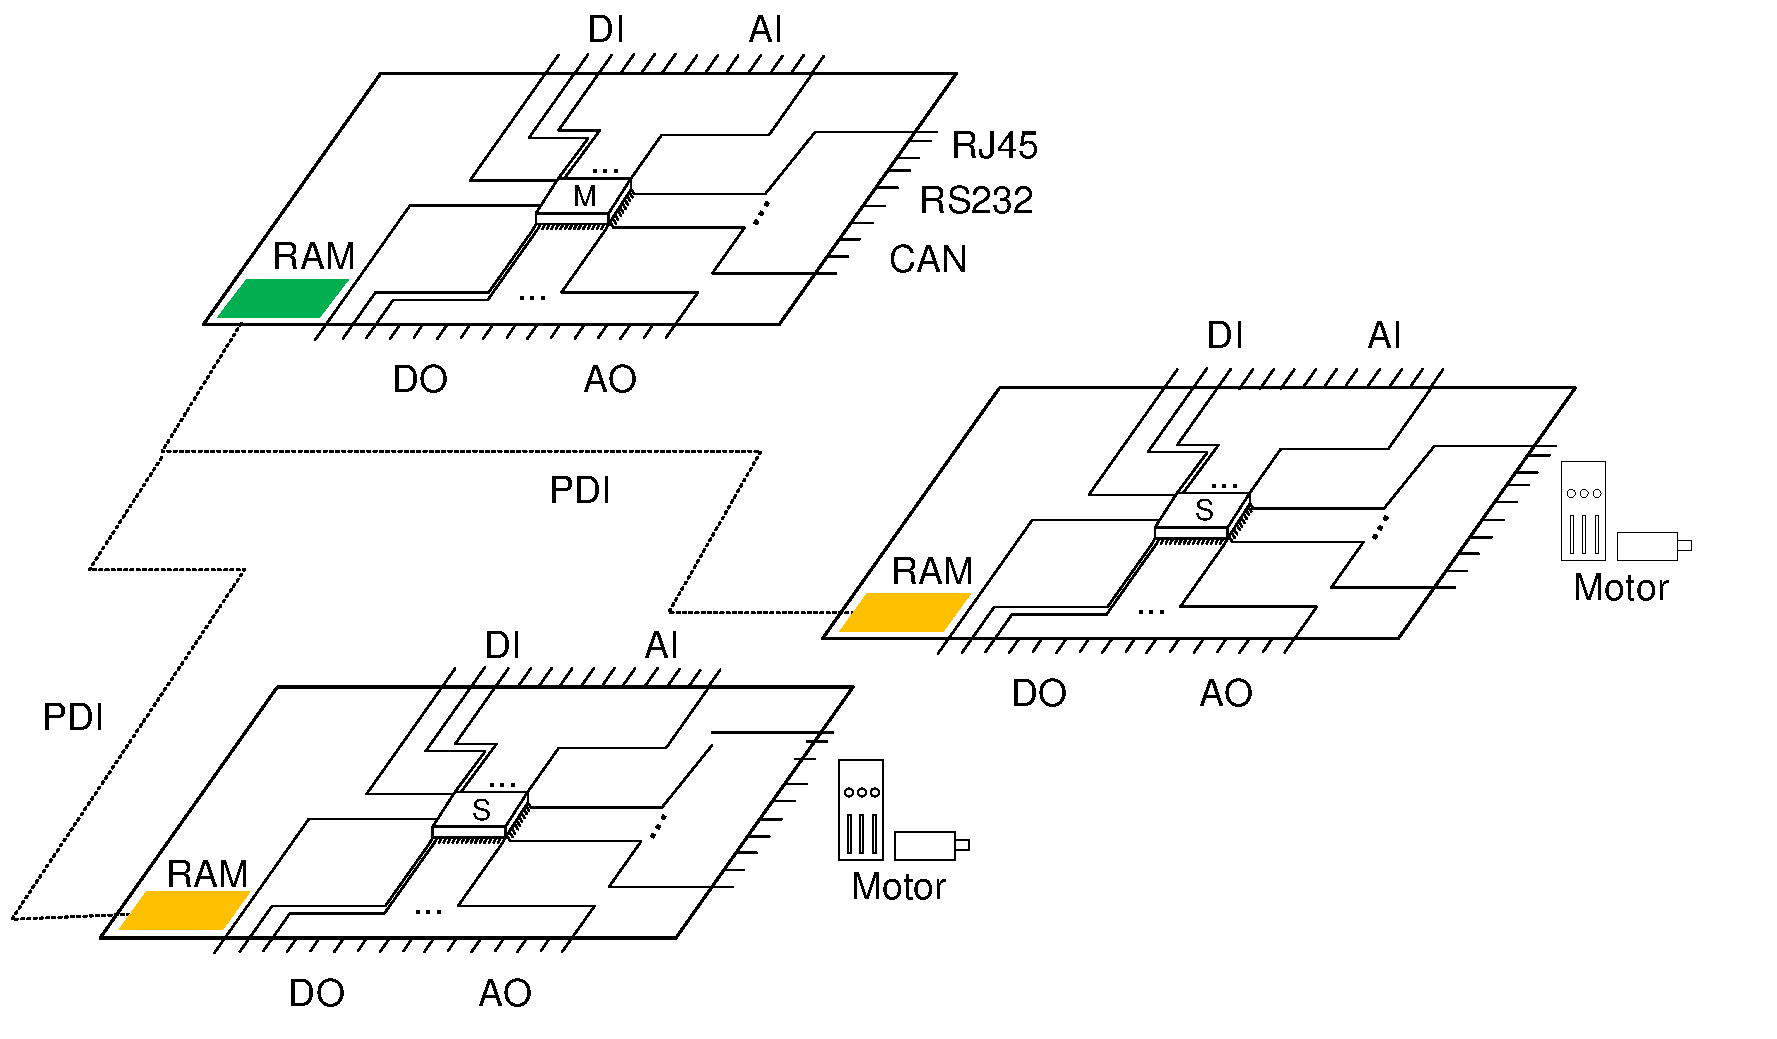
\includegraphics[width=3.5in]{fig/FIG2.pdf}
		\caption{ One type of hardware structure of multiprocessor $ePLC$ containing a master processor and two slave processors.}
		\label{fig:HardwareStructure}
	\end{figure}
	\subsection{Multi-language supported graphical component}
	\label{component}
	\begin{figure}
		\centering
		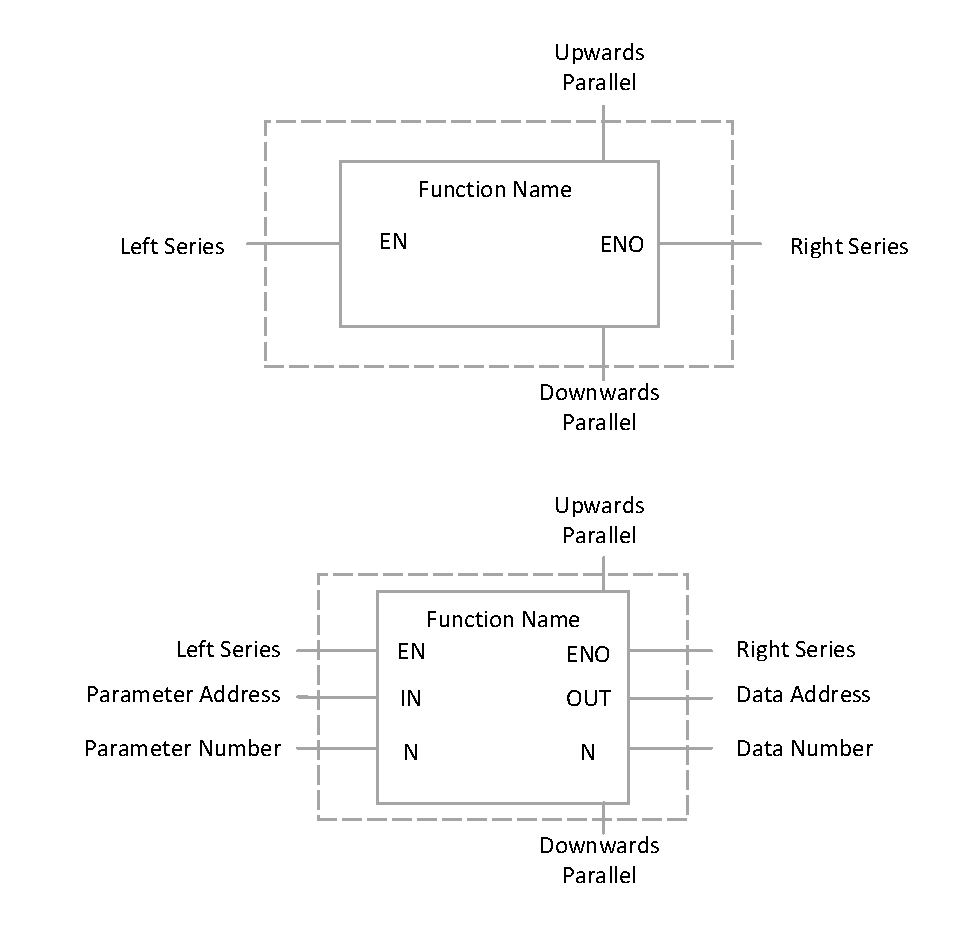
\includegraphics[width=3in]{fig/FIG6.pdf}
		\caption{ Two typical designs: single component and component with input and output.}
		\label{fig:Component}
	\end{figure}
	In order to develop the logic program and algorithm program on a uniform platform, we package the algorithm into graphical component that is multi-language-supporting. \textcolor{red}{ In technical implementation, the formal description is crucial for compiling the graphical component of the instruction list. Hence, the component is described as a 6-tuple:$\{Name,ID,PI,RI,PT,SF\}$.} Here, \textbf{Name} is the name of component used to describe the function;  \textbf{ID} is the unique identifier of the component in the graphical program; \textbf{PI} is a collection of service interfaces, including output data interfaces, right serial connection, downwards parallel connection, and some auxiliary interfaces; \textbf{RI} is a collection of requirement interfaces, including input data interfaces, left serial connection, upwards parallel connection, and some auxiliary interfaces;  \textbf{PT} is an attribute collection of the component, including position, size, comment, etc.; and \textbf{SF} is the function description explained by specific text, formula ,or frame template. The basic graphical components are divided into contact components, functional block components, coil components, cross-line vertical components, change lines, comments, etc. The multi-language component, in particular, includes the development language, the supported compiler, and the executing processor.
	
	Figure \ref{fig:Component} illustrates two component designs: a single component and a component with input and output. The single component has function name, left series, right series, upwards parallel, and downwards parallel. The component with input and output contains function name, left series, right series, upwards parallel, downwards parallel, parameter address, parameter number, data address, and data number.
	
	As shown in Fig. \ref{fig:SoftwareStructure}, from the user's point of view, after inducing the multi-language component, the algorithm and logic program could be developed in a uniform $PLC$ platform. Multi-language components are supported by multiple languages, such as IL instructions, ST language, C language, C++ language, etc. Algorithms contained in components are mainly motion control algorithms.
	\begin{figure}
		\centering
		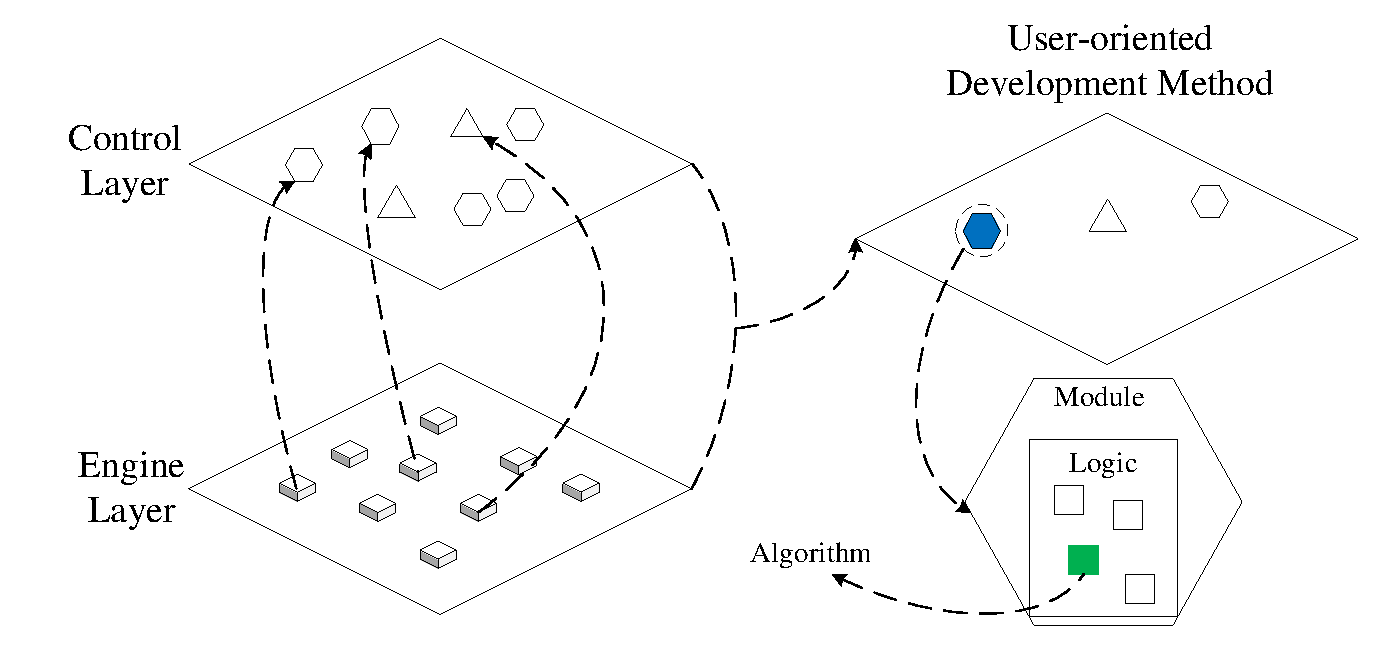
\includegraphics[width=3in]{fig/FIG3.pdf}
		\caption{ From the user's point of view, after inducing the multi-language component, the algorithm and logic program can be developed on a uniform $PLC$ platform.}
		\label{fig:SoftwareStructure}
	\end{figure}
	
	
	\begin{figure}
		\centering
		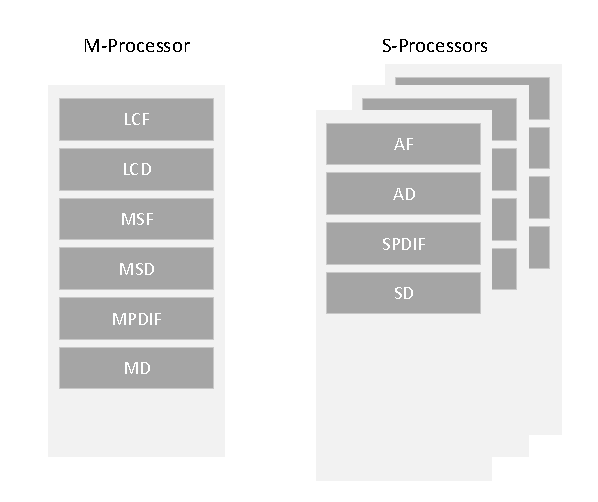
\includegraphics[width=3in]{fig/FIG4.pdf}
		\caption{ Memory allocation in master and slave processors.}
		\label{fig:Memory}
	\end{figure}
	
	\subsection{Memory Allocation}  
	
	The dedicated storage area of a $PLC$ in memory is made up of a bit data area ($M$ area) and byte data area ($D$ area). Meanwhile, we regard $M$ area and $D$ area as set $M$ of bit and set $D$ of byte. Furthermore, in the rest of this paper, if $\exists$ set $T$, we describe its subscript lower-case letter $t_i$ as an element of $T$, and the subscript $i$ is used to distinguish the elements. Henceforth, two definitions are illustrated below.
	
	\textbf{Definition 1} If $ T \subseteq M$, the value saved in $t_{i} \in \{0, 1\} $ and each element $t_i$ has four operators: $\mathcal{S}_0(t_i)$ denotes that $t_i$ is set to $0$, $\mathcal{S}_1(t_i)$ denotes that $t_i$ is set to $1$, $\mathcal{J}_0(t_i)$ represents that the value of $t_i$ is judged as $0$, and $\mathcal{J}_1(t_i)$ represents that the value of $t_i$ is judged as $1$. We then define the set $T$ as having $\mathcal{B}$ attribute.
	
	\textbf{Definition 2} If $ T \subseteq D$ and $\forall t_{i} \in T$ has 4 bytes. We define the set $T$ as having $\mathcal{D}$ attribute.
	
	
	Figure \ref{fig:Memory} shows the memory allocation of master and slave processors. All slave processors have the same storage structure.
	
	\textbf{\emph{LCF}} (Logic Control Flag Area): the flags are used to start the modules. It has $\mathcal{B}$ attribute.
	
	\textbf{\emph{LCD}} (Logic Control Data Area): these data will be used to deliver to the algorithm. It has $\mathcal{D}$ attribute.
	
	\textbf{\emph{AF}} (Algorithm Flag Area): includes the algorithm flag of execution ($AFE$) and algorithm flag of state ($AFS$). Both have $\mathcal{B}$ attribute.
	
	\textbf{\emph{AD}} (Algorithm Data Area): these data help the specified algorithm execute. It has $\mathcal{D}$ attribute.
	
	\textbf{\emph{MF}} (Message Flag Area): includes defined message flag ($DMF$) and user-customized message flag ($UMF$). $DMF$ is the necessary message for system execution, e.g., start module flag, alarm flag, etc. $UMF$ can be defined by users. Both have $\mathcal{B}$ attribute.
	
	\textbf{\emph{MD}} (Message Data Area): used to transfer message information, which includes system message data area ($DMD$) and user message data area ($UMD$). It is defined in $D$ area.
	
	\textbf{\emph{MPDIF}} (Master Processor Data Interaction Flag Area): contains begin data transfer flag from master to slave ($MSB$), transfer state of master from master to slave ($MSF$), acknowledge flag of master from master to slave ($MSA$), and transfer state of master from slave to master ($MSS$). All have $\mathcal{B}$ attribute.
	
	\textbf{\emph{MSD}} (Master Processor Data Interaction Data Area): an area that stores the data delivered from slave processors. It has $\mathcal{D}$ attribute.
	
	\textbf{\emph{SPDIF}} (Slave Processor Data Interaction Flag Area): includes the begin data transfer flag from slave to master ($SMB$), transfer state of slave from slave to master ($SMF$), acknowledge flag of slave from slave to master ($SMA$), and transfer state of slave from master to slave ($SMS$). All have $\mathcal{B}$ attribute.
	
	\textbf{\emph{SMD}} (Slave Processor Data Interaction Data Area): stores the data delivered from master processor. It has $\mathcal{D}$ attribute.
	
	\subsection{User-oriented Thread Design}
	From the user's point of view, in most cases, the logic control program ($LCP$) and algorithm program ($AP$) can be developed independently \cite{wu2018customized}; hence, we have a logic thread and algorithm thread. However, in order to satisfying the ever-growing performance requirements of users, we proposed the customized multiprocessor $ePLC$. Correspondingly, an individual motion thread is designed into every slave processor. The user-oriented thread structure can be seen in Fig \ref{fig:Threads}. Every processor is a four-level pre-emptive scheduling thread structure: \textbf{Emergent Thread}, \textbf{Communication Thread}, \textbf{Diagnose Thread}, and \textbf{APC Thread} as seen in \cite{wu2018customized}. Two special threads are explained below.
	
	\textbf{Control Thread}: runs in the master processor and has functions including dealing with DI$\backslash$O, executing logic program, exchanging data with slave processors, etc.
	
	\textbf{Algorithm Thread}: runs in the slave processor and contains functions including interacting data with master, executing algorithm program, controlling actuators, etc.
	
	\subsection{\textcolor{red}{Formal Description of Software Structure}}  
	\textcolor{red}{Normally, the software structure could be divided into two-layer structure: a control layer for the logic program and a motion layer for the motion control. In addition, considering the advantage of complexity reduction in modular design \cite{Vyatkin2013Software}, we therefore provide a system-level frame for modular design. Hence, the software structure with modular design is depicted in Fig. \ref{fig:SoftwareStructure}.} The program is composed of many modules, and a module consists of a logic program and several related algorithms. Modules work under mechanisms: reasonable memory allocation, $LPM$ interaction, with a data mechanism, and running multi-threading. \textcolor{red}{For a clearer description, we can define an $ePLC$ program as follows}:
	
	\begin{equation}
	\left\{
	\begin{array}{l}
	PS = \{MS, MA , LPM, TD\},\\
	ms_i \in MS = \{lcp_i, \bigcup_{j=g}^h ap_j\},\\
	lcp_i \in LCP = \{ip_i, lcf_i, lcd_i, lpb_i\},\\
	ap_j \in AP = \{afe_j, afs_j, ad_j, ab_j\}.
	\end{array}
	\right.
	\end{equation}
	
	The programming structure ($PS$) consists of modules ($MS$), memory allocation ($MA$), $LPM$ data interaction, and threads ($TD$). Each $ms_i$ has two parts: a logic control program $lcp_i$ and several algorithm programs ($ap_g, ap_{g+1},..., ap_{j},..., ap_{h}$). Each $lcp_i$ includes an initial program ($ip_i$), logic control flag ($lcf_i$), logic control data ($lcd_i$), and logic program body ($lpb_i$). Each $ap_{j}$ contains $afe_{j}$, $afs_{j}$, $ad_{j}$, and algorithm body ($ab_{j}$).
	
	\begin{figure}
		\centering
		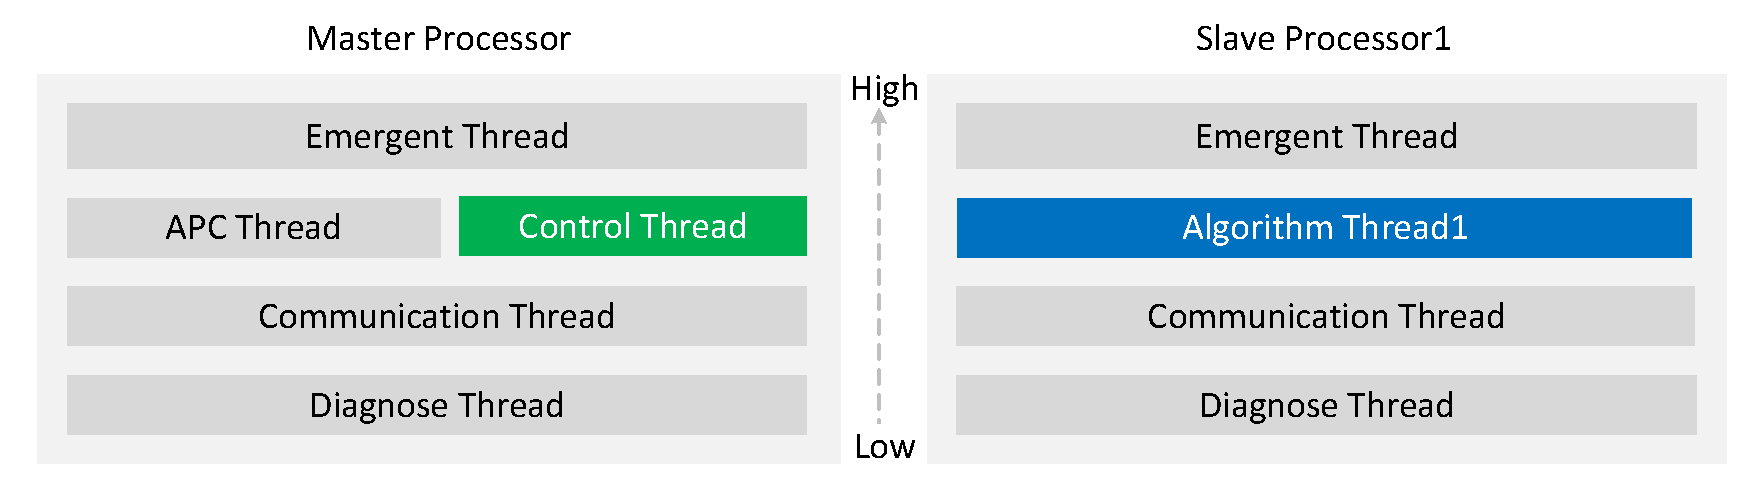
\includegraphics[width=3in]{fig/FIG5.pdf}
		\caption{ User-oriented thread design in master and slave processors.}
		\label{fig:Threads}
	\end{figure}
	\section{System Implementation}
	\label{Process}
	\subsection{Compilation of graphic program}
	The compilation of the graphic program contains two parts: 1) compiling the graphic language into instruction list, and 2) compiling the multi-language components.
	
	In the first part, since we see the multi-language components as a common component, the compilation of graphic language embedded multi-language components is almost the same as the process of \cite{Yan2010Compiling}, in which readers can find a detailed explanation. \textcolor{red}{As shown in Fig. \ref{fig:Compile},} we adopt three steps to implement the first of the two above-mentioned compilations:
	
	\textbf{Step 1}: Convert topology structure to directed graph according to LD syntax library and analyze the errors of the topology.
	
	\textbf{Step 2}: Generate a binary decomposition tree according to series and parallel rules.
	
	\textbf{Step 3}: Generate IL instructions according to the IL grammar library. For multi-language components, it is described as a program entry.
	
	\begin{figure}
		\centering
		\includegraphics[width=3in]{fig/Compile.pdf}
		\caption{Three steps in compilation of graphic program, which contains multi-language component: 1) convert topology structure to directed graph, 2) generate a binary decomposition tree, and 3) generate IL instructions.}
		\label{fig:Compile}
	\end{figure}
	
	In the second part, the multi-language components are compiled. For the convenience of users, they can still use the same grammar to program the $ePLC$ dedicated storage area inside the multi-language component, such as $M2000=1$, which represents giving $1$ to the bit area $M2000$, whereas it is illegal in other languages. Hence, we should compile the component to the identifiable code which contains the following two steps:
	
	\textbf{Step 1}: Address mapping. Every type of processor has its own address mapping rules ($AMR$), e.g.,
	\begin{eqnarray}
	APR = \{CID, MAS, DAS, \mathcal{A}_m, \mathcal{A}_d\},
	\end{eqnarray}
	where $CID$ is the compiler identity and $MAS$ and $DAS$ are the start address of $M$ and $D$ areas, respectively. $\mathcal{A}_m$ and $\mathcal{A}_d$ are the rules for mapping $M$ and $D$ to the address of the processor, respectively, see Algorithms \ref{alg1} and\ref{alg2}. Algorithm \ref{alg1} translates the four operators of each element $m_i$, which are $\mathcal{S}_0(m_i)$, $\mathcal{S}_1(m_i)$, $\mathcal{J}_0(m_i)$, and $\mathcal{J}_1(m_i)$, to recognizable the form of the $CID$ compiler. In addition, in the $PLC$ platform, we adopt the octal system, so it is necessary to translate the octal number to a decimal number. Algorithms \ref{alg1} and \ref{alg2} both contain this process.
	
	
	\textbf{Step 2}: Call the corresponding compiler to compile the component.
	
	
	\begin{algorithm}
		\label{alg1}
		\caption{$\mathcal{A}_m$}%算法名字
		%\LinesNumbered %要求显示行号
		\KwIn{string oStr of $m_i$ contained its operator}%输入参数
		\KwOut{converted string cStr}%输出
		Get the number $i$ from oStr\; 
		Get operator $opt$ from oStr\;
		remainder r = $i\%10$\;
		Octal oI =  $i/10$\;
		Convert oI to decimal dI\; 
		\For{opt}{
			\If{opt==$\mathcal{S}_0$}{
				cStr = "CassMen[$MAS$+dI] $\gg$ r == 0"\;
			}
			\If{opt==$\mathcal{S}_1$}{
				cStr = "CassMen[$MAS$+dI] $\gg$ r == 1"\;
			}		
			\If{opt==$\mathcal{J}_0$}{
				cStr = "CassMen[$MAS$+dI] $\mid \sim$(1 $\ll$ r)"\;
			}
			\If{opt==$\mathcal{J}_1$}{
				cStr = "CassMen[$MAS$+dI] \& (1 $\ll$ r)"\;
			}	  	    
		}
	\end{algorithm}
	\begin{algorithm}
		\label{alg2}
		\caption{$\mathcal{A}_d$}%算法名字
		%\LinesNumbered %要求显示行号
		\KwIn{string oStr of $d_i$}%输入参数
		\KwOut{converted string cStr}%输出
		Get the number $i$ from oStr\; 
		Convert $i$ to decimal dI\; 
		cStr = "CassMen[$DAS$+dI]"\;
	\end{algorithm}
	
	
	
	\subsection{LPM data interaction}
	\textcolor{red}{In order to implement data interaction among different parts and processors, we propose the $LPM$-data-interaction method.} As shown in Fig. \ref{fig:Interaction}, we define the $LPM$ data interaction as having three parts: $\mathcal{L}$ (layer data interaction), $\mathcal{P}$ (processor data interaction), and $\mathcal{M}$ (module data interaction). $\mathcal{L}$ seen in \cite{wu2018customized} is the process of exchanging the data between the application-customized layer and control layer.
	
	$\mathcal{P}$ is used to establish the data interaction between master processor and slave processors; hence, it contains the process of transferring data from master to slave ($\mathcal{P}_{mts}$) and the process of transferring data from slave to master ($\mathcal{P}_{stm}$), both of which are defined as follows:
	\begin{equation}
	\left\{
	\begin{array}{l}
	\mathcal{P}_{mts} = \mathcal{U} (msb_i,msf_i,sma_i,sms_i,smd_i),\\
	\mathcal{P}_{stm} = \mathcal{U} (smb_i,smf_i,msa_i,mss_i,msd_i),
	\end{array}
	\right.
	\end{equation}
	where $\mathcal{U}$ is the function that implements the process of data interaction between master and slave processors. $\mathcal{P}_{mts}$ and $\mathcal{P}_{mts}$ use the same function $\mathcal{U}$.
	
	The process flow of $\mathcal{P}_{mts}$ is expressed  as follows:
	$\mathcal{S}_1(msb_i)\to\mathcal{S}_1(msf_i)\to send(smd_i)\to\mathcal{S}_0(msb_i)\to\mathcal{S}_1(sms_i)\to check(smd_i)\to\mathcal{S}_1(sma_i)\to\mathcal{S}_0(sms_i)\to\mathcal{S}_0(sma_i)\to\mathcal{S}_0(msf_i)$.
	
	Here, $send(msd_i)$ denotes sending data to $msd_i$ in the slave processor. $check(msd_i)$ denotes checking the  data of $msd_i$. $\to$ denotes the transition to the next step, e.g., $\mathcal{S}_1(msb_i)\to\mathcal{S}_1(msf_i)$ denotes that $msb_i$ and is set one, and then $msf_i$ is set one.
	
	$\mathcal{M}$ is used to establish the data interaction among modules. It includes two types of messages: system-defined message interaction $\mathcal{M}_{d}$ and user message interaction $\mathcal{M}_{u}$. The process is defined as follows:
	\begin{equation}
	\left\{
	\begin{array}{l}
	\mathcal{M}_{d} = \mathcal{V} (dmf_i,dmd_i,\mathcal{E}),\\
	\mathcal{M}_{u} = \mathcal{V} (umf_i,umd_i\,\mathcal{E}),
	\end{array}
	\right.
	\end{equation}
	where $\mathcal{V}$ is the function used to broadcast messages and transfer data, $\mathcal{E}$ is the collection of all execution functions after receiving a related message, and $\mathcal{M}_{s}$ and $\mathcal{M}_{u}$ have the same function $\mathcal{V}$.
	
	One module receives a system-defined message as follows:
	$\mathcal{J}_1(smf_i)\to GetMessage_{j}(dmf_i)\to GetData(dmd_i)\to\mathcal{E}_j$.
	
	Here, $GetMessage_{j}(dmf_i)$ represents the $i$th module receiving a message $dmf_i$ and $GetData(dmd_i)$ represents the $i$th module receiving the message information.
	
	\begin{figure}
		\centering
		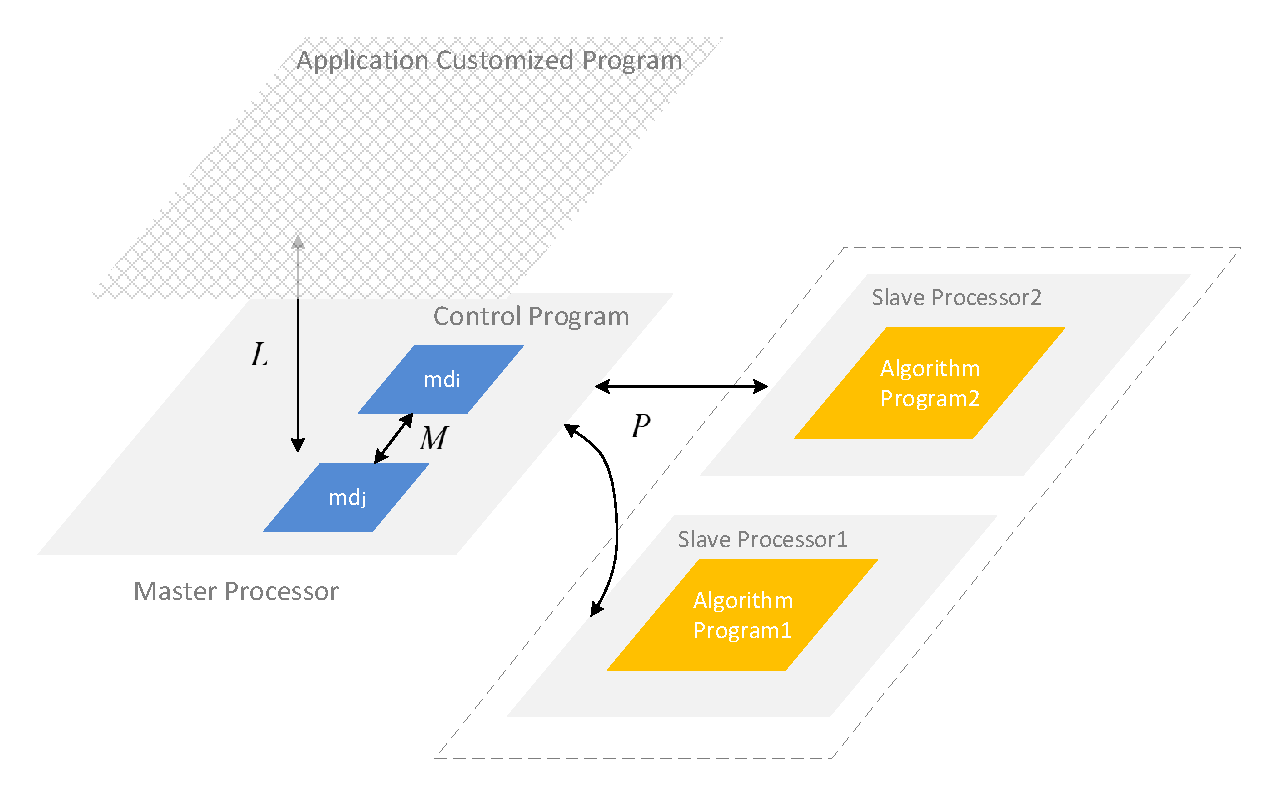
\includegraphics[width=3in]{fig/Interaction.pdf}
		\caption{ $LPM$ data interaction defined as having three parts: $\mathcal{L}$ (layer data interaction), $\mathcal{P}$ (processor data interaction), and $\mathcal{M}$ (module data interaction).}
		\label{fig:Interaction}
	\end{figure}
	
	\subsection{Execution of threads}
	Commonly, threads in master processor and in slave processors execute separately according to their priority, and the interaction between control thread and algorithm threads occurs when using $\mathcal{P}_{mts}$ and $\mathcal{P}_{mts}$. Basic execution units of control thread are as follows:
	
	\textbf{$C_{1}$}: start a module.
	
	\textbf{$C_{2}$}: transfer data to slave processor by $\mathcal{P}_{mts}$.
	
	\textbf{$C_{3}$}: deal with the feedback data.
	
	\textbf{$C_{4}$}: broadcast a message.
	
	\textbf{$C_{5}$}: handle the message.
	
	A motion thread contains the following basic execution units:
	
	\textbf{$M_{1}$}: start the algorithm.
	
	\textbf{$M_{2}$}: execute the algorithm.
	
	\textbf{$M_{3}$}: feedback the data to master processor by $\mathcal{P}_{stm}$.
	
	\textbf{$M_{4}$}: end algorithm.
	
	Two cases shown in Fig. \ref{fig:threadFlow} are explained below:
	
	\textbf{Case 1}: Execution of a control thread and two algorithm threads among three processors. The control thread ($CT$) traverses $LCF$, finds $ms_i$ to be executed , runs $lcp_i$, finds $ap_j$, executes $C_1$ unit, executes $C_2$ unit, and then transfers data from $LCD$ to $SMD$ of processor 1. Algorithm thread ($AT$) 1 executes $M_1$ unit, executes $M_2$ after transferring data from $SMD$ to $AD$, runs $M_3$ unit, and feedbacks data to $CT$. When $ap_j$ finishes, $AT$ 1 executes $M_4$ and informs $CT$ of the end of $ap_j$. $CT$ executes $C_3$ to end the process and then finds $ap_{j+1}$, executes $C_1$ and $C_2$, transfers the data from $LCD$ to $SMD$ of processor 2, $AT$ 2 executes $M_1$ unit, and executes $M_2$ after transferring data from $SMD$ to $AD$. When $ap_{j+1}$ finishes, $AT$ 2 executes $M_4$ unit and informs $CT$ of the end of $ap_{j+1}$. $CT$ executes $C_3$ to finish the process.
	
	\textbf{Case 2}: Execution of control thread and two algorithm threads among three processors together with message mechanism. The $CT$ traverses $LCF$, finds $ms_i$ to be executed , runs $lcp_i$, finds $ap_j$, executes $C_1$ unit, executes $C_2$ unit, and then transfers data from $LCD$ to $SMD$ of processor 1. $AT$ 1 executes $M_1$ unit and executes $M_2$ after transferring data from $SMD$ to $AD$. During the execution of $ms_i$, $CT$ executes $C_4$ to broadcast the message $dmf_x$ to inform $ms_{k}$ to run. After execution of $C_5$, $ms_{k}$ obtains data and starts, and then $CT$ finds $ap_{j+1}$ in $ms_{k}$, executes $C_1$ and $C_2$, transfers the data from $LCD$ to $SMD$ of processor 2, $AT$ 2 executes $M_1$ unit, and executes $M_2$ after transferring data from $SMD$ to $AD$. During the execution of $ap_{j+1}$, $AT$ 1 executes $M_4$ and informs $CT$ to execute $C_3$. After that, $ap_{j+1}$ finishes, and then $CT$ executes $C_3$ to finish the process.
	
	
	
	\begin{figure}
		\centering
		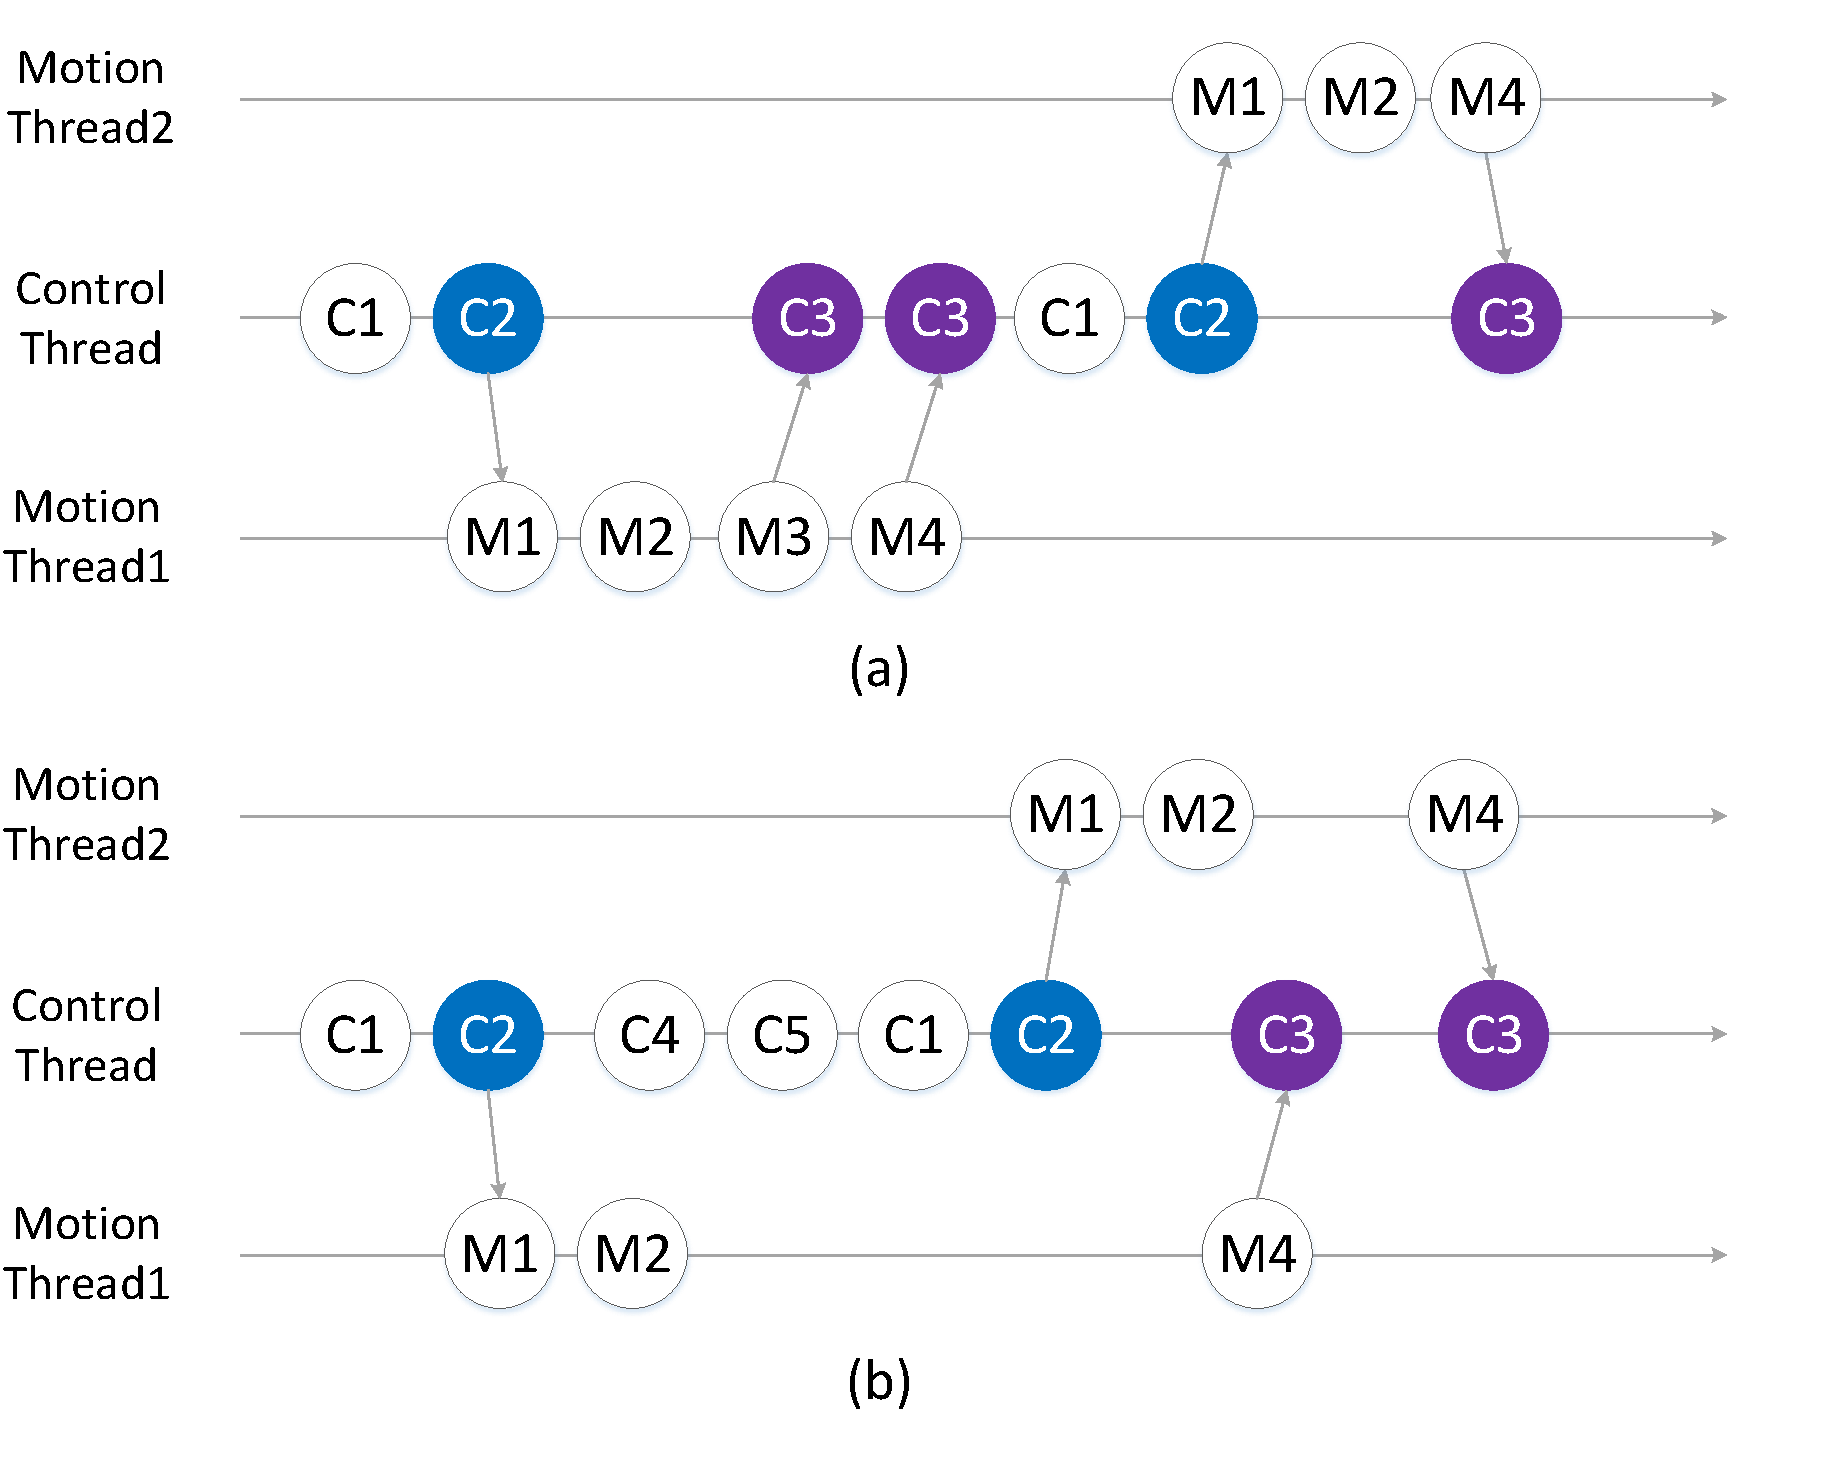
\includegraphics[width=3in]{fig/threadFlow.pdf}
		\caption{ Execution of control thread and two algorithm threads among three processors with and without messages.}
		\label{fig:threadFlow}
	\end{figure}
	\subsection{Finite state machines}
	The finite state machines adopt the 5-tuple, which is similar to\cite{Hierons2016Parallel}:
	\begin{equation}
	\mathcal{F} = (Q, X, Y, \delta, \lambda),
	\end{equation}
	where $Q = \{q_0, q_1,..., q_i\}$ is the collection of states, $q_0 \in Q$ is the initial state, $X$ is the finite set of inputs, $Y$ is the finite set of outputs, and $\delta$ is the state transition function $\delta: Q\times X \rightarrow Q$. $\lambda$ is the output function $\lambda: Q\times X\rightarrow Y$. If $F$ is in state $q$ and $x$ occurs, then $F$ transitions to state $q' = \delta(q, x)$ and outputs $y = \lambda(q, x)$. This transition is denoted $\tau = (s,x/o,s')$.
	
	Hence, we have the following finite state machines of the master processor:
	\begin{equation}
	\label{FMaster}
	\left\{
	\begin{array}{l}
	\mathcal{F}_{m} = \{Q_m, X_m, Y_m,\delta_m, \lambda_m\},\\
	Q_m = \{mstop, mrun, mbm, pdi\},\\
	X_m = \{x_{m1}, x_{m2}, x_{m3}, x_{m4}, x_{m5}, x_{m6}, x_{m7}\},\\
	Y_m = \{y_{m1}, y_{m2}, y_{m3}\},
	\end{array}
	\right.
	\end{equation}
	where $mstop$ is the stop state and the initial state of master processor, $mrun$ is the run state, $mbm$ is the broadcast state, and $pdi$ is the data interaction state. The inputs are defined as follows:
	\begin{align}
	\notag x_{m1}&\Leftrightarrow \exists lcf_i: \mathcal{J}_1(lcf_i),\\
	\notag x_{m2}&\Leftrightarrow  \forall lcf_i: \mathcal{J}_0(lcf_i),\\
	\notag x_{m3}&\Leftrightarrow \exists mf_i: \mathcal{J}_1(mf_i),\\
	\notag x_{m4}&\Leftrightarrow \forall mf_i: \mathcal{J}_0(mf_i),\\
	\notag x_{m5}&\Leftrightarrow \exists msf_i, mss_j: \mathcal{J}_1(msf_i) \lor \mathcal{J}_1(mss_j),\\
	\notag x_{m6}&\Leftrightarrow \forall msf_i, mss_j, mf_k: \mathcal{J}_0(msf_i) \land \mathcal{J}_0(mss_j) \land \mathcal{J}_0(mf_k),\\
	\notag x_{m7}&\Leftrightarrow \forall msf_i, mss_j, \exists mf_k: \mathcal{J}_0(msf_i) \land \mathcal{J}_0(mss_j) \land \mathcal{J}_1(mf_k),\\
	\notag y_{m1}&\Leftrightarrow C_1,\\
	\notag y_{m2}&\Leftrightarrow C_4,\\
	\notag y_{m3}&\Leftrightarrow C_2\quad or\quad C_3.
	\end{align}
	Here, e.g., $x_{m1}\Leftrightarrow \exists lcf_i: \mathcal{J}_1(lcf_i)$ denotes that $x_{m1}$ is an input of $X_m$ and this input is equivalent to the existence of a logic control flag $lcf_i$ whose value is 1.
	
	We than can obtain the state transitions of the master processor:
	\begin{equation}
	\left\{
	\begin{array}{l}
	\tau_m1 = (mstop, x_{m1}/y_{m1}, mrun),\\
	\tau_m2 = (mrun, x_{m2}, mstop),\\
	\tau_m3 = (mrun, x_{m3}/y_{m2}, mbm),\\
	\tau_m4 = (mbm, x_{m4}, mrun),\\
	\tau_m5 = (mrun, x_{m5}/y_{m3}, pdi),\\
	\tau_m6 = (pdi, x_{m6}, mrun),\\
	\tau_m7 = (mbm, x_{m5}/y_{m3}, pdi),\\
	\tau_m8 = (pdi, x_{m7}, mbm).\\
	\end{array}
	\right.
	\end{equation}
	
	
	The finite state machines of every slave processor are as follows:
	\begin{equation}
	\label{FSlave}
	\left\{
	\begin{array}{l}
	\mathcal{F}_{s} = \{Q_s, X_s, Y_s, \delta_s, \lambda_s\},\\
	Q_s = \{sstop, sready, srun, pdi\},\\
	X_s = \{x_{s1}, x_{s2}, x_{s3}, x_{s4}, x_{s5}\},\\
	Y_s = \{y_{s1}, y_{s2}, y_{s3}\},\\
	\end{array}
	\right.
	\end{equation}
	where $sstop$ is the stop state and the initial state, $srun$ is the run state, $sready$ is the ready state, and $pdi$ is the data interaction state. The events are defined as follows:
	\begin{align}
	\notag x_{s1}&\Leftrightarrow \exists sms_i: \mathcal{J}_1(sms_i),\\
	\notag x_{s2}&\Leftrightarrow \exists afe_i: \mathcal{J}_1(afe_i),\\
	\notag x_{s3}&\Leftrightarrow \exists afs_i: \mathcal{J}_1(afs_i),\\
	\notag x_{s4}&\Leftrightarrow \forall afs_i: \mathcal{J}_0(afs_i),\\
	\notag x_{s5}&\Leftrightarrow \exists smb_i, sms_j: \mathcal{J}_1(smb_i) \lor \mathcal{J}_1(sms_j),\\
	\notag y_{s1}&\Leftrightarrow M_1,\\
	\notag y_{s2}&\Leftrightarrow M_2,\\
	\notag y_{s3}&\Leftrightarrow M_3.
	\end{align}
	
	
	We then can obtain the state transitions of the slave processor:
	\begin{equation}
	\left\{
	\begin{array}{l}
	\tau_{s1} = (sstop, x_{s1}/y_{s1}, pdi),\\
	\tau_{s2} = (pdi, x_{s2}, sready),\\
	\tau_{s3} = (sready, x_{s3}/y_{s2}, srun),\\
	\tau_{s4} = (srun, x_{s4}, sstop),\\
	\tau_{s5} = (srun, x_{s5}/y_{s3}, pdi).
	\end{array}
	\right.
	\end{equation}
	
	Figure \ref{fig:state} illustrates all of the finite state machines of $ePLC$, which contains master processor $M$, slave processor $S_1$, and slave processor $S_i$. This is the graphical form of Eqs. \ref{FMaster} and \ref{FSlave}. 
	\begin{figure}
		\centering
		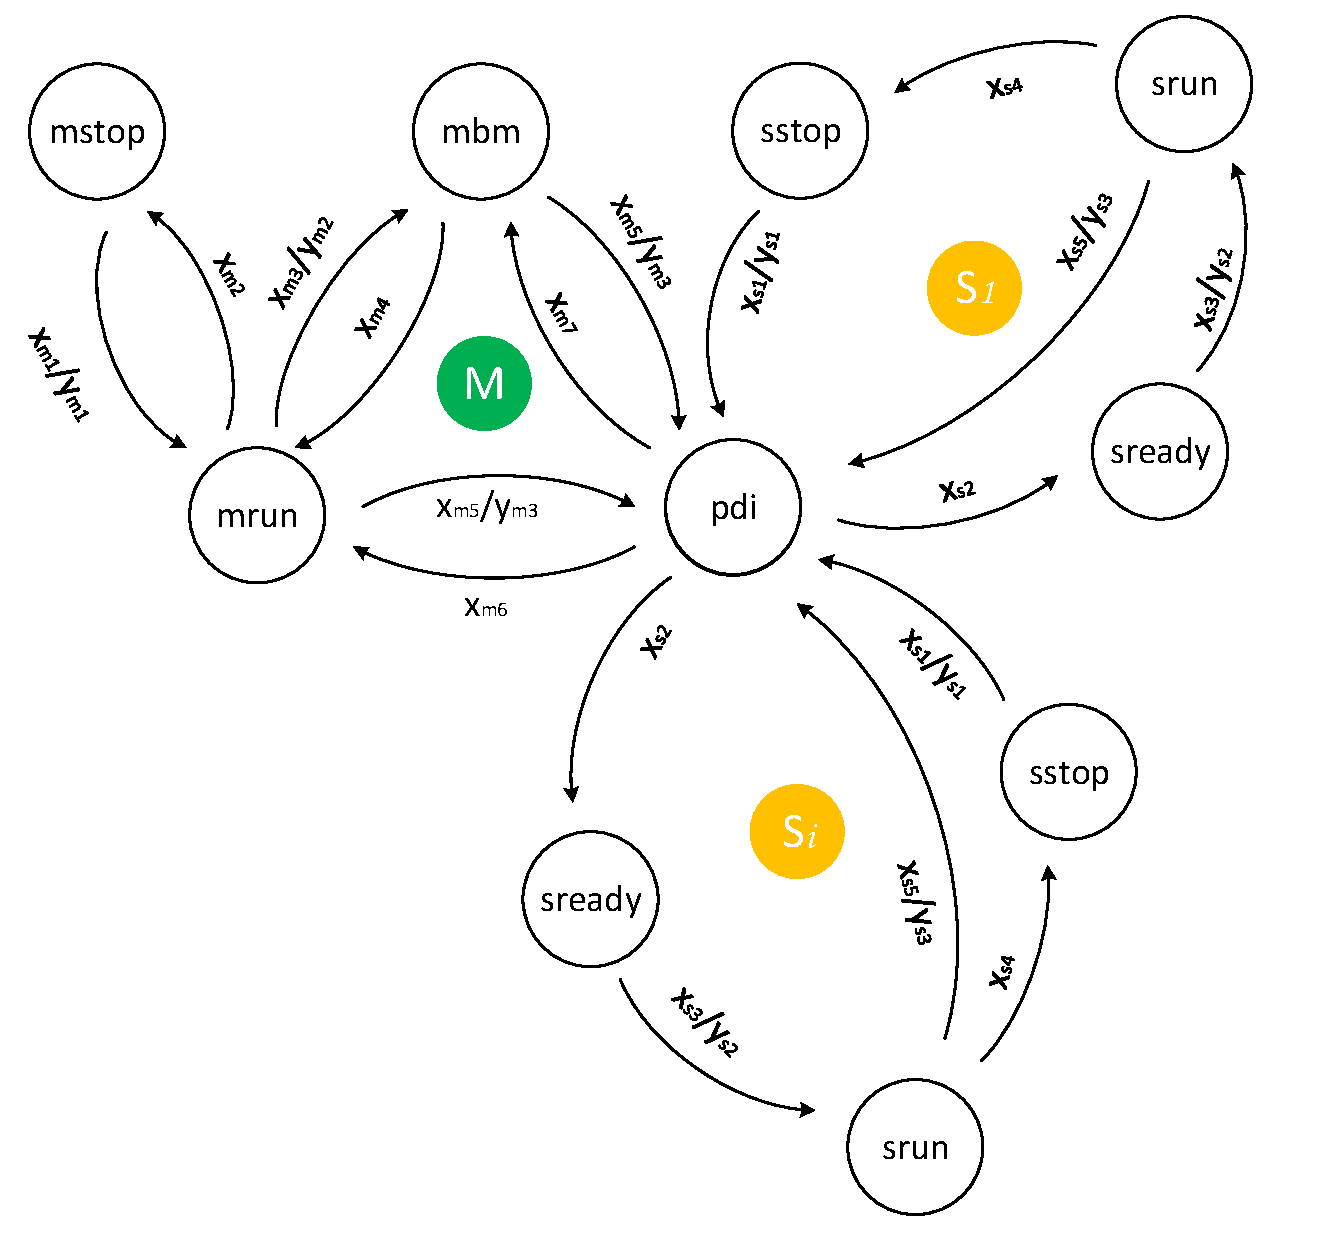
\includegraphics[width=3in]{fig/state.pdf}
		\caption{ Finite state machines of $ePlC$, which contains master processor $M$, slave processor $S_1$, and slave processor $S_i$.}
		\label{fig:state}
	\end{figure}
	\section{Experiment}
	\label{Experiment}
	
	\begin{figure}
		\centering
		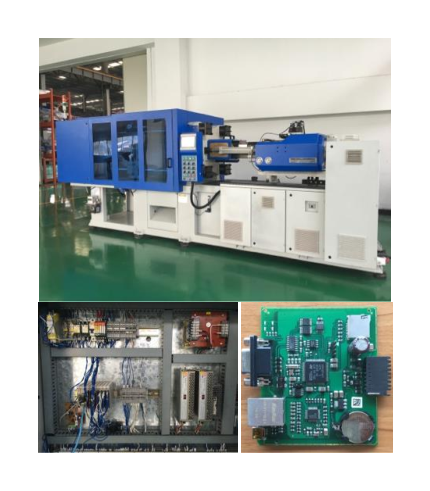
\includegraphics[width=3in]{fig/FIG10.pdf}
		\caption{200-T IMM and multiprocessor $ePLC$.}
		\label{fig:IMM}
	\end{figure}
	
	\subsection{Distributed control system}
	As shown in Fig. \ref{fig:IMM}, we verified the proposed development method on a 200-T $IMM$. The TI F28M35 chip was chosen as the main chip of the $ePLC$. It has two cores: a TI C28x and an ARM Cortex M3. Considering the DSP is more suitable for motion control, the Cortex M3 is chosen as the master processor and C28x as the slave processor. The $ePLC$ has an RS232 and a CAN. The RS232 is used to download programs and connect with the HMI, and the CAN is designed to extend the DI$\backslash$O and AI$\backslash$O. The $HMI$ can be customized by users.
	
	\subsection{Software structure}
	Figure \ref{fig:ld} shows the uniform development platform that we devised. The dotted-line box of Fig. \ref{fig:ld} (a) represents the C-language component and Fig. \ref{fig:ld} (b) its partial code. This component represents to output a small velocity and pressure in setup mode.
	
	After the design of every used component, we designed the modules according to Table \ref{table:IMMSystem}. Additionally, a special module was designed to control the execution flow of all modules with the $DMF$ and $DMD$.
	
	\begin{figure}
		\centering
		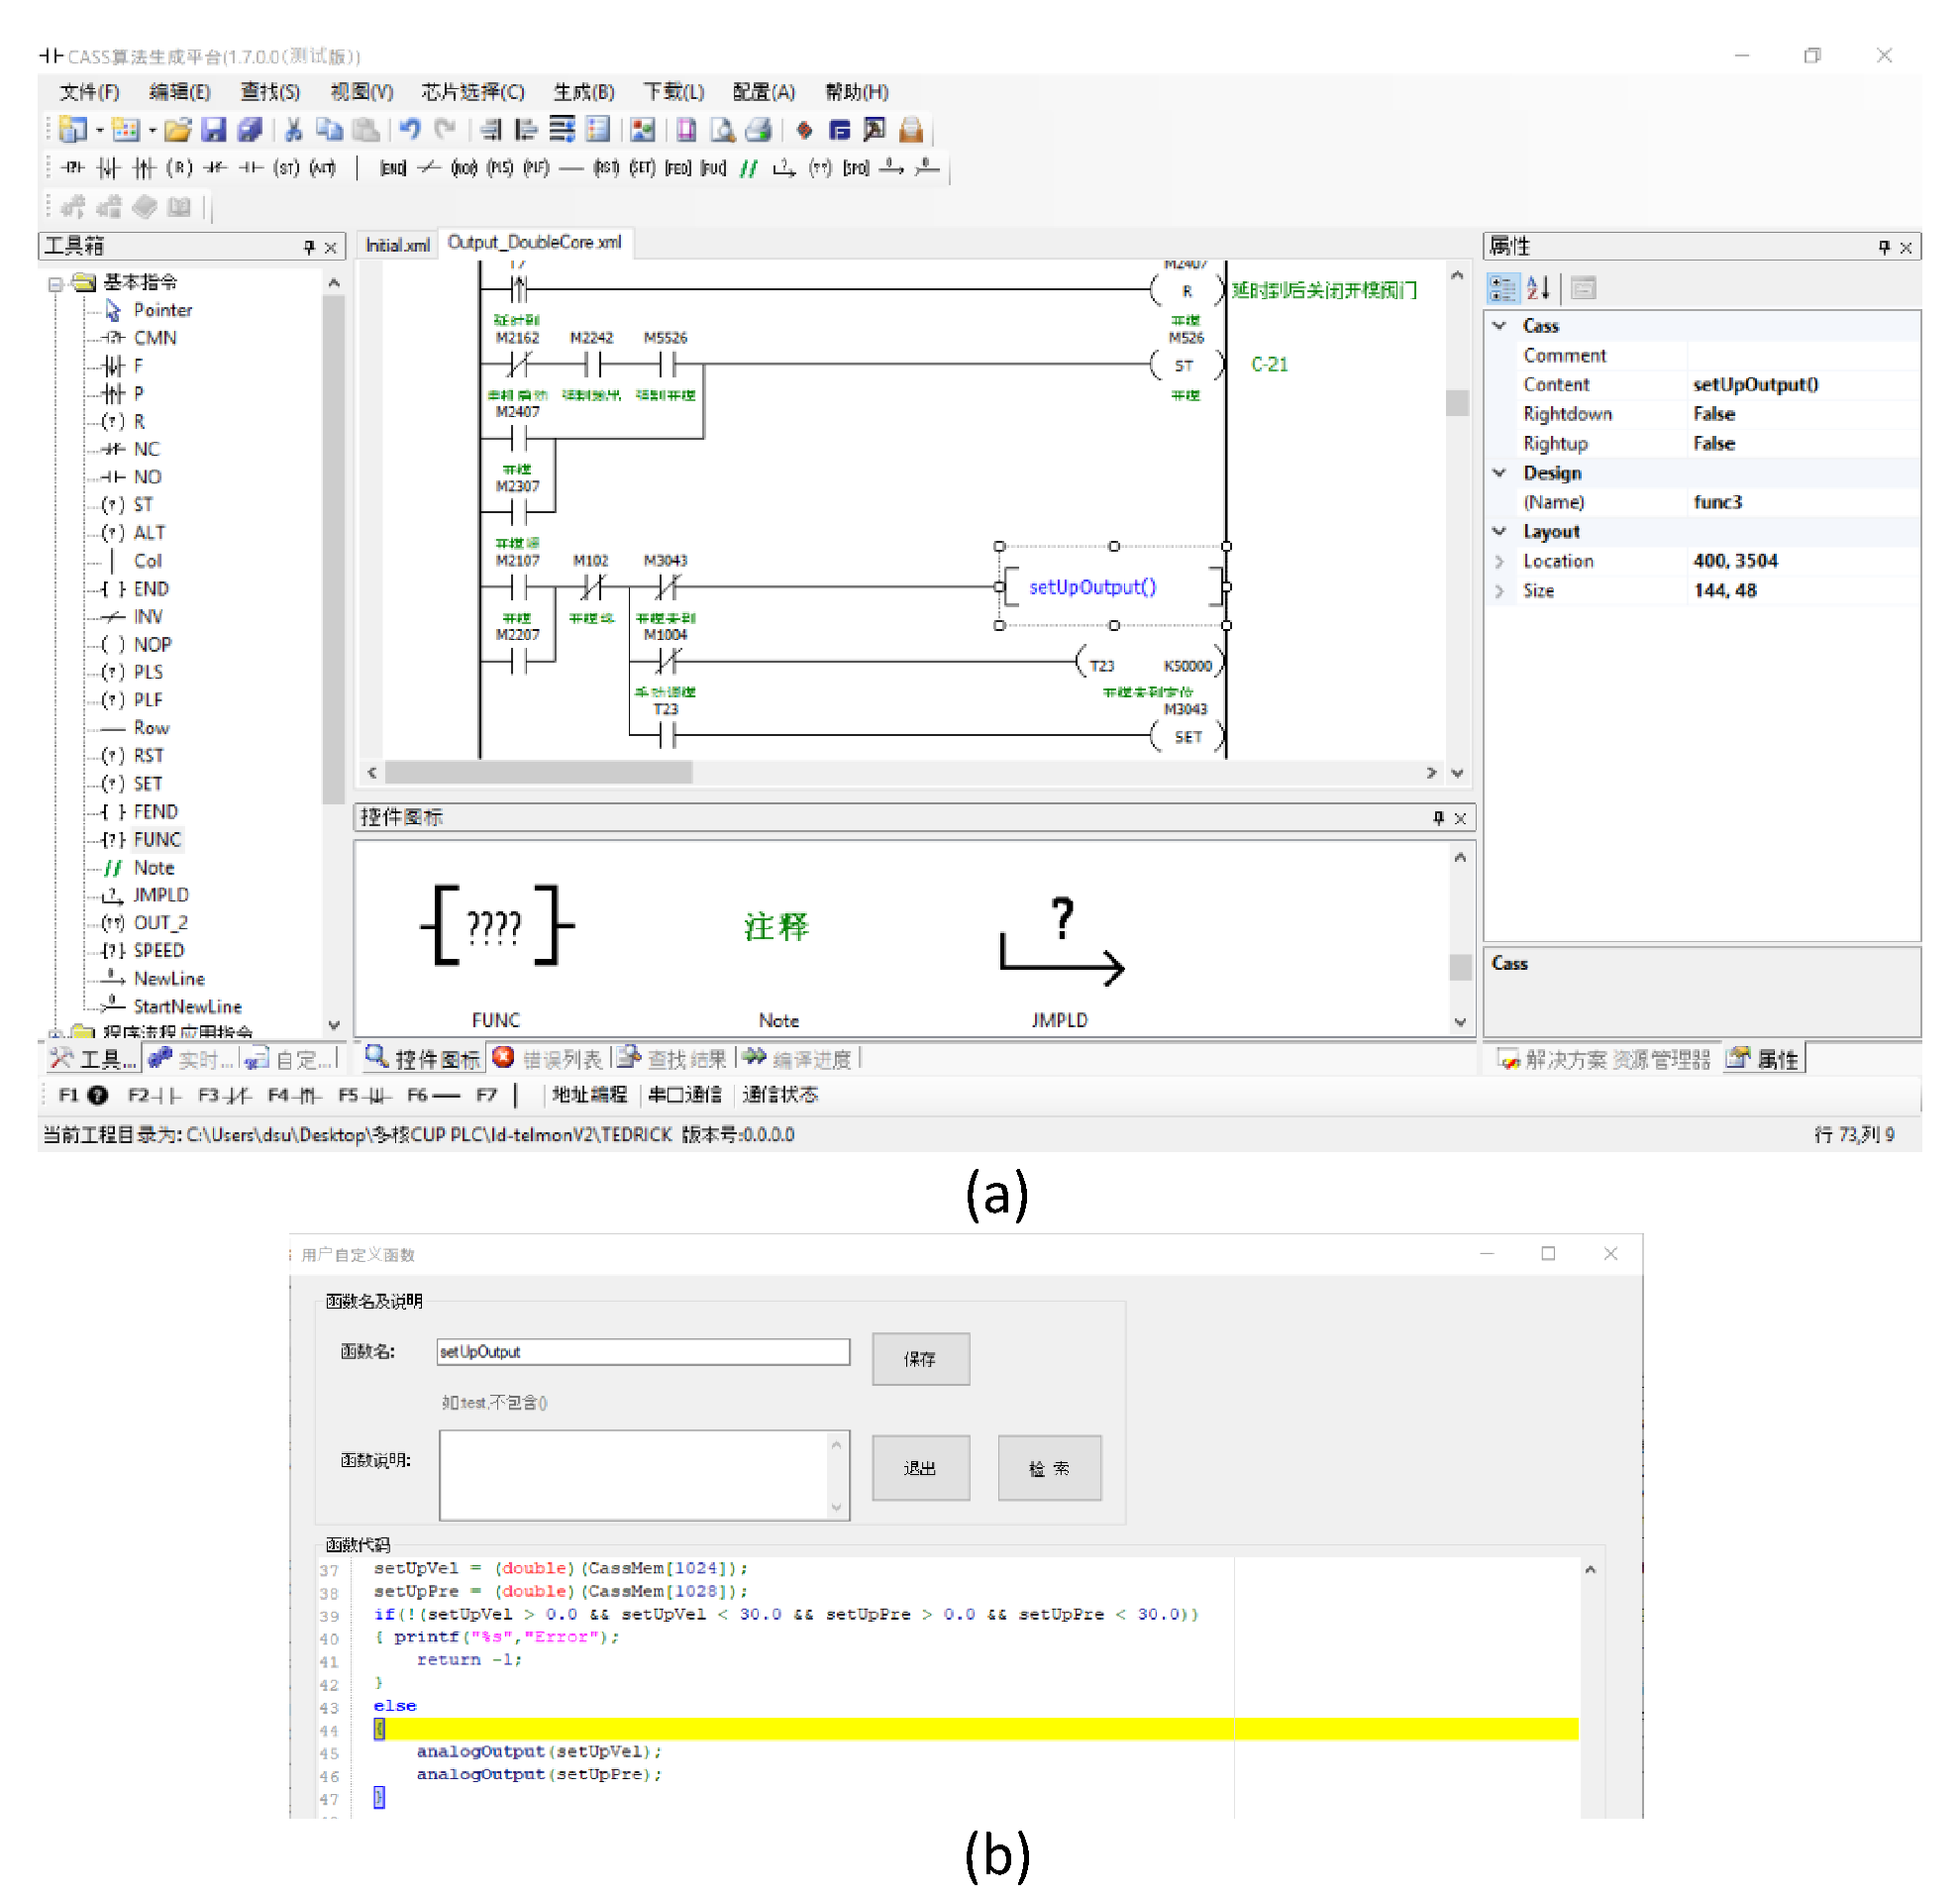
\includegraphics[width=3in]{fig/ld.pdf}
		\caption{(a) uniform development platform with C-language component in dotted-line box and (b) its partial code. This component represents to output a small velocity and pressure in setup mode.}
		\label{fig:ld}
	\end{figure}
	
	Three typical requirements for using the proposed user-oriented development method are as follows:
	\begin{enumerate}
		\item Using multiprocessors: Add S-curve acceleration and deceleration algorithms. For this case, we ran the S-curve in the DSP (slave processor).
		\item Design in the uniform development platform: Add an ejector module containing a T-curve. We designed the $LCP$ with $LD$ and the T-curve packaged as a component in the same platform.
		\item Modular design: Inject before high pressure of the mold closes. We customized a message flag in $MSF$ and broadcast the message at the beginning of high pressure, after which the injection module received the message and the $CT$ started it.
	\end{enumerate}
	\subsection{Analysis}
	We compared the system information, development method, and key performance indicators among the TECHMATION system, the KEBA system, and the proposed system. The compared controller types of the KEBA and TECHMATION systems are i1000 and TE-CH2, respectively. 
	
	\begin{enumerate}
		\item System information. The TECHMATION and KEBA systems account for the majority of market share. \textcolor{red}{As shown in Table \ref{table:systemComparison}, the KEBA and TECHMATION systems have more powerful CPUs and more RAM than the implemented system. The main frequency of the KEBA and TECHMATION systems are 400 and 80 MHz, respectively, and their RAM 128 MB and 512 kB, respectively. In contrast, the main frequency and RAM of the implemented system are 72 MHz and 132 kB, respectively.} Owing to the reduced complexity, our system can have a customized $PLC$ and separate $HMI$. To some extent, this lowers the cost significantly. The proposed system adopts the widely used distributed structure, which decreases wire usage and increases resistance to interference.
		\item Development method. Our system adopted a user-oriented development method, including a customized multiprocessor $ePLC$, component-based uniform development platform, and comprehensive optimization of the system. It is difficult to achieve these in other systems and they cannot support a C-language component. In particular, the TECHMATION system is developed by assembly instruction and does not support IEC61131-3.
		\item Key performance indicators. With our best knowledge, we adopted defective percentage ($DP$), error of change-over position ($ECP$), error of cushion minimum ($ECM$), error of charging end position ($ECEP$), and error of mold open end position ($EMOEP$) as the key performance indicators. All the systems were adjusted to use a T-curve and the key parameters were set to the same value. The cycle time, mold close time, mold open time, injection time, charging and cooling time, and ejector forward time and ejector backward time were controlled at approximately 8, 2, 2, 1, 1, 1, 0.5, and 0.5 s, respectively. Figure \ref{fig:Compare} shows the 100-times error line graph of the key performance indicators. The proposed system has nearly identical performance as the KEBA system, which is better than that of the TECHMATION system. Table \ref{table:IMMSystem} shows the comparison of startup time ($ST$), $DP$, and the mean of the key performance indicators. The proposed system's startup time was increased by more than 5 times in the case of almost identical key performance.
	\end{enumerate}

	\begin{table}
		\scriptsize \caption{\textcolor{red}{System information comparison}}
		\label{table:systemComparison}
		\begin{center}
			\begin{threeparttable}
			\renewcommand{\arraystretch}{1.4}
			\setlength\tabcolsep{3pt}
			%\begin{tabular}{|p{2cm}|p{1.5cm}|p{1.5cm}|p{2.3cm}|p{2.3cm}|p{2.3cm}|p{2cm}|}
			\begin{tabular}{|l|c|c|c|c|}	
				\hline
				            &Controller model &CPU     &Main frequency       &RAM\\
				\hline
				KEBA        &Series i1000     &PowerPC &400 MHz              &128 MB  \\
				\hline
				TECHMATION  &TE-CH2           &DSP54    &80 MHz              &512 kB  \\
				\hline
				Implemented &-                &F28M35  &72 MHz\tnote{1} &132 kB\tnote{2} \\
				\hline			
			\end{tabular}
			\begin{tablenotes}
			\footnotesize
			\item[1] \textcolor{red}{Main frequencies of ARM and DSP are 100 and 150 MHz, respectively.}
			\item[2] \textcolor{red}{Value is the summation of RAM, DSP, and shared RAM.}
			\end{tablenotes}
			\end{threeparttable}
		\end{center}
	\end{table}
	\begin{table}
		\scriptsize \caption{Key performance comparison}
		\label{table:ComparisonG}
		\begin{center}
		\begin{threeparttable}
			\renewcommand{\arraystretch}{1.4}
			\setlength\tabcolsep{3pt}
			%\begin{tabular}{|p{2cm}|p{1.5cm}|p{1.5cm}|p{2.3cm}|p{2.3cm}|p{2.3cm}|p{2cm}|}
			\begin{tabular}{|l|c|c|c|c|c|c|}
				\hline
				Brand & ST &DP&$\overline{ECP}$ \tnote{3}&$\overline{ECM}$&$\overline{ECEP}$ &$\overline{EMOEP}$\\
				\hline
				TECHMATION  & 27 s  &0.27\% &0.094 & 0.2 & 0.13 & 0.17 \\
				\hline
				KEBA        & 72 s  &0.24\% &0.064 & 0.1 & 0.1 & 0.12 \\
				\hline
				Implemented   & 5 s     &0.25\% &0.05 & 0.1 & 0.11 & 0.11\\
				\hline
			\end{tabular}
			\begin{tablenotes}
			\footnotesize
			\item[3] \textcolor{red}{$\overline{ECP}$ denotes the 100-time mean of ECP.}
		    \end{tablenotes}
		\end{threeparttable}
	\end{center}
	\end{table}
		\begin{figure}
		\centering
		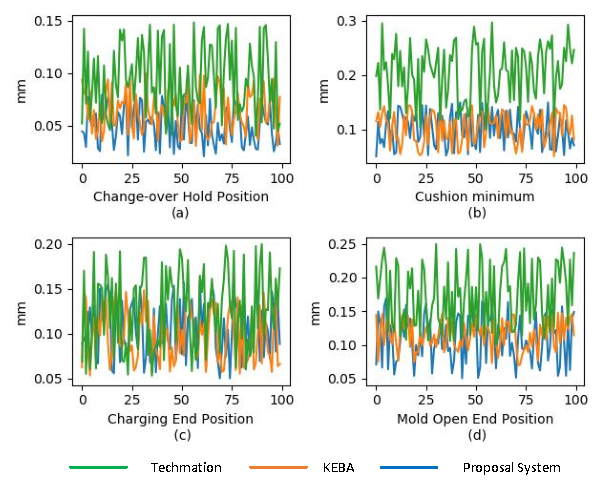
\includegraphics[width=3in]{fig/Compare.pdf}
		\caption{(a) is ECP, (b) is ECP, (c) is ECM, (d) is EMOEP.}
		\label{fig:Compare}
	\end{figure}

	\section{Conclusions}
	\label{conclusion}
	In this paper, we presented a user-oriented development method in which a customized multiprocessor $ePLC$ was proposed to enhance performance, a multi-language-supporting graphical component was proposed to improve the adaptability of developers, and an optimized system structure (reasonable memory allocation, user-oriented thread structure, $LPM$ data interaction, modular software design, and finite state machines) was proposed to reduce the developmental complexity. Ultimately, we adopted the proposed method to implement a distributed $IMM$ system. Through comparison with the TECHMATION and KEBA systems, our system startup time increased by more than 5 times in the case of almost identical key performance. Furthermore, our system supports a customized multiprocessor $ePLC$ and detached $HMI$. 
	
	\textcolor{red}{In planned additional work, more applications will be implemented to prove the system's robustness. Meanwhile, integration with other systems (e.g., a visual system) will be undertaken to study the system flexibility.} 
	
	
	
	
	
	\ifCLASSOPTIONcaptionsoff
	\newpage
	\fi
	
	
	
	% trigger a \newpage just before the given reference
	% number - used to balance the columns on the last page
	% adjust value as needed - may need to be readjusted if
	% the document is modified later
	%\IEEEtriggeratref{8}
	% The "triggered" command can be changed if desired:
	%\IEEEtriggercmd{\enlargethispage{-5in}}
	
	% references section
	
	% can use a bibliography generated by BibTeX as a .bbl file
	% BibTeX documentation can be easily obtained at:
	% http://www.ctan.org/tex-archive/biblio/bibtex/contrib/doc/
	% The IEEEtran BibTeX style support page is at:
	% http://www.michaelshell.org/tex/ieeetran/bibtex/
	%\bibliographystyle{IEEEtran}
	% argument is your BibTeX string definitions and bibliography database(s)
	%\bibliography{IEEEabrv,../bib/paper}
	%
	% <OR> manually copy in the resultant .bbl file
	% set second argument of \begin to the number of references
	% (used to reserve space for the reference number labels box)
	
	\bibliographystyle{IEEEtran}
	\bibliography{reference}
	
	% biography section
	%
	% If you have an EPS/PDF photo (graphicx package needed) extra braces are
	% needed around the contents of the optional argument to biography to prevent
	% the LaTeX parser from getting confused when it sees the complicated
	% \includegraphics command within an optional argument. (You could create
	% your own custom macro containing the \includegraphics command to make things
	% simpler here.)
	%\begin{IEEEbiography}[{\includegraphics[width=1in,height=1.25in,clip,keepaspectratio]{mshell}}]{Michael Shell}
	% or if you just want to reserve a space for a photo:
	
	
	
	
	
	% insert where needed to balance the two columns on the last page with
	% biographies
	%\newpage
	
	
	% You can push biographies down or up by placing
	% a \vfill before or after them. The appropriate
	% use of \vfill depends on what kind of text is
	% on the last page and whether or not the columns
	% are being equalized.
	
	%\vfill
	
	% Can be used to pull up biographies so that the bottom of the last one
	% is flush with the other column.
	%\enlargethispage{-5in}
	
	
	
	% that's all folks
\end{document}


